\documentclass[11pt,oneside,a4paper]{article}
\usepackage{graphicx}
\usepackage{booktabs}
\usepackage{caption}
\usepackage{subcaption}
\usepackage{amsmath}
\usepackage{amsfonts}
\usepackage{amssymb}
\usepackage{lscape}
\usepackage{psfrag}
\usepackage[usenames]{color}
\usepackage{bbm}
\usepackage[update]{epstopdf}
\usepackage[bookmarks,pdfstartview=FitH,a4paper,pdfborder={0 0 0}]{hyperref}
\usepackage{verbatim}
\usepackage{listings}
\usepackage{textcomp}
\usepackage{fancyhdr}
\usepackage{multirow}
\usepackage{tikz}
\usepackage{lipsum}
\usepackage{xcolor}
\usepackage{wrapfig}
\usepackage[margin=1in]{geometry}
\usepackage{ccicons}
\newcommand{\hint}[1]{{\color{blue} \em #1}}

\makeatletter
\def\cleardoublepage{\clearpage\if@twoside \ifodd\c@page\else%
\hbox{}%
\thispagestyle{empty}%
\clearpage%
\if@twocolumn\hbox{}\clearpage\fi\fi\fi}
\makeatother

\title{Advanced Topics in Communication Networks}
\author{Yannick Merkli, \texttt{ymerkli@ethz.ch}}
\date{ETH Zurich, HS 2019}

\begin{document}
	
\begin{titlepage}
\maketitle
\vspace{3cm}
\thispagestyle{empty}


\begin{abstract}
	\noindent This document is a "lecture summary" style script that closely follows the slides of the \textit{Advanced Topics in Communication Networks} lecture  at ETH Zurich \cite{advnet}. The contribution to this is editing and refactoring as well as providing additional material for better understanding. This summary was created during the fall semester 2019. Due to updates to the syllabus content, some material may no longer be relevant for future versions of the lecture.\\
	Most graphics are copy \& pasted from the slides. If you don't want yours here, please contact me and I will remove them. Otherwise, this work is published as CC BY-NC-SA.
	
	\begin{center}
		\ccbyncsa
	\end{center}
	
	\noindent I do not guarantee correctness or completeness, nor is this document endorsed by the lecturers. Feel free to point out any erratas. For the full \LaTeX \ source code, consider \texttt{\href{https://github.com/ymerkli/eth-summaries}{github.com/ymerkli/eth-summaries}}.
\end{abstract}

\end{titlepage}

\maketitle
\thispagestyle{empty}
\raggedbottom
\clearpage

\pagenumbering{roman}

\clearpage
\setcounter{tocdepth}{2}
\tableofcontents
\clearpage
\pagenumbering{arabic}

\section{Introduction}

Networking is on the verge of a paradigm shift towards deep programmability.

\subsection{The network managment crisis}
Networks are large distributed systems running a set of distributed algorithms. These algorithms produce the forwarding state which drives IP traffic to its destination. Operators adapt their network behavior by configuring each network device individually. This is extremely tedious and error-prone with a single mistyped line being enough to bring down an entire network (fat-thumbing). Further, the complexity in networks keeps increasing with more and more protocols appearing, a lot of which are badly documented (read an RFC and find out).

\subsection{Software-defined networking (SDN)}

SDN tries to design network control and is predicated around two simple concepts: (1) Separate the control-plane from the data-plane. (2) Provide an API to directly access the data-plane.\\
In traditional computer networks, each networked device has a local control-plane. SDN allows to have a central control-plane, controlling multiple networked devices at once. This has several advantages: (1) Simpler management, (2) Faster pace of innovation, (3) Easier interoperability, (4) Simpler, cheaper equipment. Having a common open, vendor-agnostic interface enables a control plane to control forwarding devices from different hardware and software vendors. OpenFlow does exactly this: OpenFlow is essentially an API to a switch flow table. The OpenFlow interface started simple, with the abstraction of a single table of rules that could match packets on a dozen header fields (e.g., MAC addresses, IP addresses, protocol, TCP/UDP port numbers, etc.). Over the past five years, the specification has grown increasingly more complicated, with many more header fields and multiple stages of rule tables, to allow switches to expose more of their capabilities to the controller. So essentially, the OpenFlow protocol became too complex.

\subsection{Deep network programmability}

Deep network programmability tries to adopt the good ideas of OpenFlow while solving its shortcomings. OpenFlow's problem is that it's  not flexible enough for a highly dynamic environment such as networking, with constantly changing protocols and specifications.
Future switches should support flexible mechanisms for parsing packets and matching header fields, allowing controller applications to leverage these capabilities through a common, open interface. Recent chip desings show that such flexibility can be achieved in custom ASICs at terabit speeds.

\begin{figure}[hb]
	\centering
	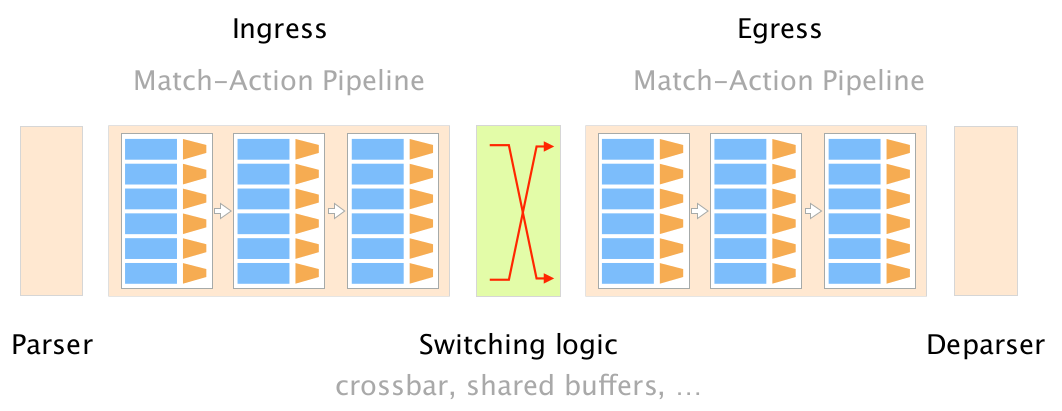
\includegraphics[width=0.75\textwidth,scale=1]{figures/PISA}
	\caption{Protocol Independent Switch Architecture (PISA) for high-speed programmable packet forwarding. \cite{advnet}}
	\label{fig:PISA}
\end{figure}

\newpage

\begin{figure}%[hb]
	\centering
	\begin{subfigure}[t]{.5\textwidth}
		\centering
		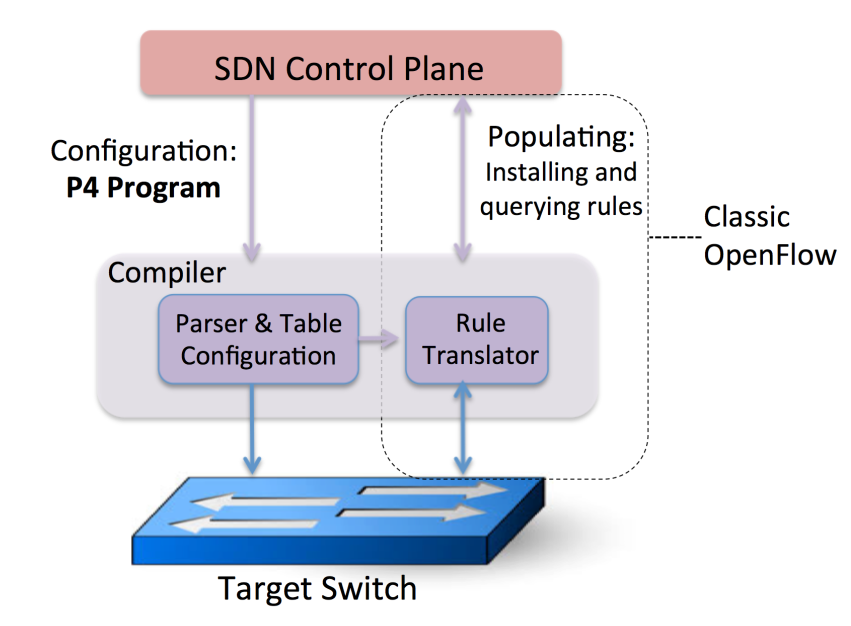
\includegraphics[width=\linewidth]{figures/P4_overview}
		\label{fig:P4_overview}
	\end{subfigure}%
	\begin{subfigure}[t]{.5\textwidth}
		\centering
		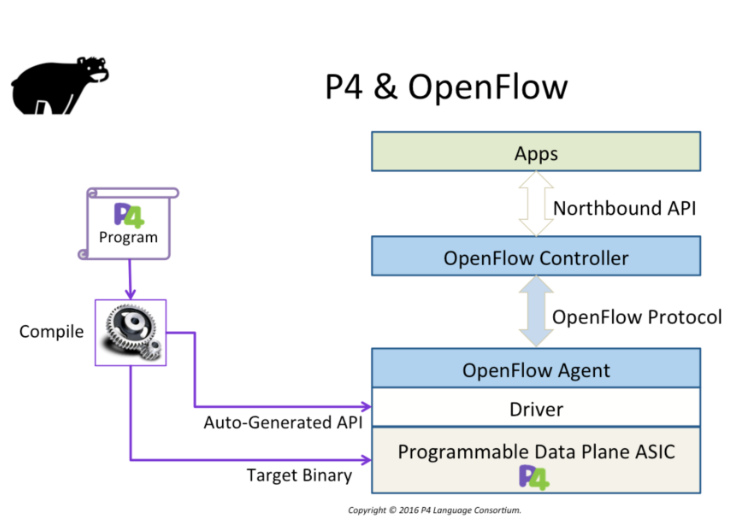
\includegraphics[width=\linewidth]{figures/P4_openflow}
		\label{fig:P4_openflow}
	\end{subfigure}
	\caption{P4 is a language to configure switches. \cite{bosshart2014p4}}
\end{figure}


Each chip has its own low-level interface, however this might vary for different hardware. Ideally we would want a higher-level language which can be used to configure a switch. This is exactly what P4 (Programming Protocol-independent Packet Processors) does: P4 is a higher-level language which is used to configure a switch, telling it how packets are to be processed. P4 can further be used with existing APIs (such as OpenFlow) that are designed to populate the forwarding tables in fixed function switches.

\section{The P4 programing language}

P4 raises the level of abstraction for programming the network, and can serve as a general interface between the controller and the switches. As such, P4 tries to achieve the following three main goals:
\vspace{-\topsep}
\begin{itemize}
	\setlength{\itemsep}{0pt}
	\setlength{\parskip}{0pt}
	\item Reconfigurability. The controller should be able to redefine the packet parsing and processing in the field.
	\item Protocol independence. The switch should be able to specify (i) a packet parser (ii) a collection of match-action tables that process theses headers.
	\item Target independence. The P4 program should run on various hardware with the compiler producing the target-dependent program.
\end{itemize}
\vspace{-\topsep}

\noindent A P4 program consists of three basic parts: Parser, match-action pipeline, deparser. In this course, we rely on a simple $P4_{16}$ switch architecture (v1model).

\begin{figure}[hb]
	\centering
	\begin{subfigure}[t]{.5\textwidth}
		\centering
		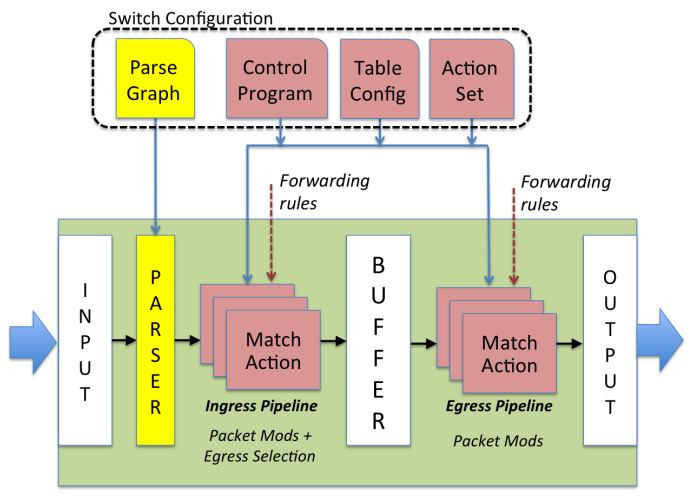
\includegraphics[width=\linewidth]{figures/forwarding_model}
		\caption{The abstract P4 forwarding model. \cite{bosshart2014p4}}
		\label{fig:forwarding_models}
	\end{subfigure}%
	\begin{subfigure}[t]{.5\textwidth}
		\centering
		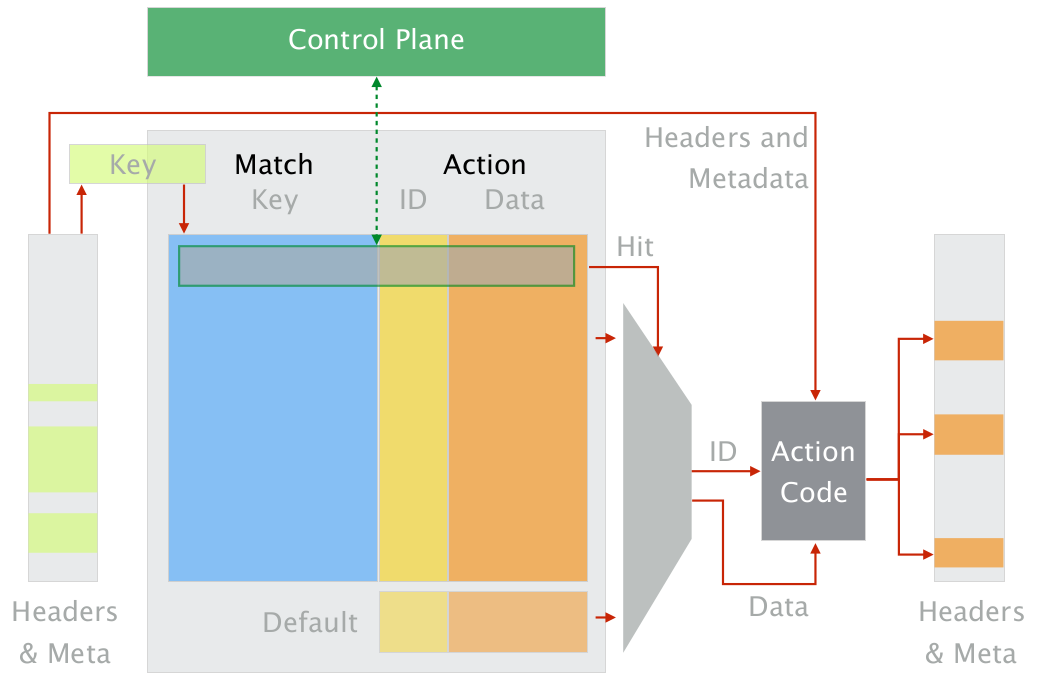
\includegraphics[width=\linewidth]{figures/match_action_tables}
		\caption{Reconfigurable match-action table. \cite{advnet}}
		\label{fig:match_action_tables}
	\end{subfigure}
\end{figure}

\newpage

\noindent The forwarding model is controlled by two types of operations: Configure and Populate. Configure operations program the parser, set the order of match + action stages, and specify the header fields processed by each stage. Configuration determines which protocols are supported and how the switch may process packets. Populate operations add (and remove) entries to the match-action tables that were specified during configuration. Population determines the policy applied to packets at any given time.

\subsection{Language specification}
\subsubsection{Data types}

$P4_{16}$ is a statically typed language with base types and operators to derive composed ones. Base types are:

\begin{center}
	\begin{tabular}{ |c|c| } 
		\hline
		bool & Boolean value \\ 
		\hline
		bit\textless W\textgreater & Bit-string of width W \\ 
		\hline
		int\textless W\textgreater & Signed integer of width W \\ 
		\hline
		varbit\textless W\textgreater & Bit-string of dynamic length $\leq W$ \\
		\hline
		match\textunderscore kind & describes ways to match table keys \\
		\hline
		error & used to signal errors \\
		\hline
		void & no values, used on few restricted instances \\
		\hline
	\end{tabular}
\end{center}
\noindent Note that there are no floats or strings.\newline

Headers are composed operators. Headers are similar to structs in C, containing different fields. Parsing a packet using \texttt{extract()} fills in the fields of the header from a network packet. Headers further have a hidden "validity" field which is set to true upon a successful \texttt{extract()}.

\begin{figure}[hb]
	\centering
	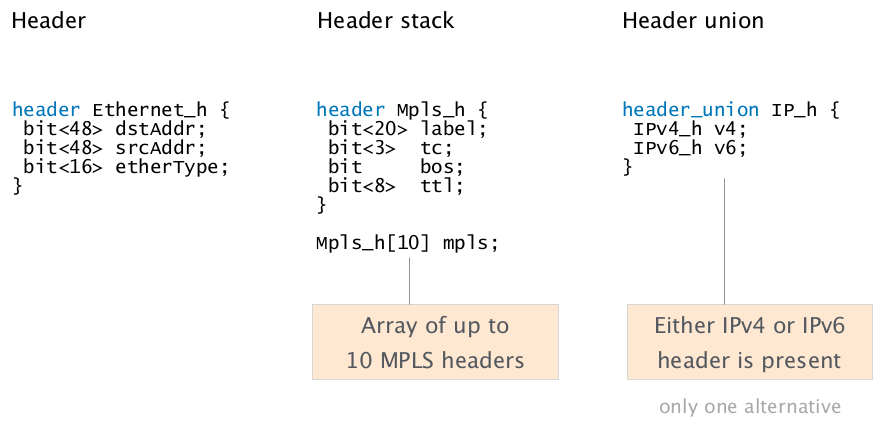
\includegraphics[width=0.75\textwidth,scale=1]{figures/headers}
	\label{fig:headers}
	\cite{advnet}
\end{figure}

\subsubsection{Operations}\label{operations}

P4 operations are similar to C operations and vary depending on the types (unsigned/signed ints, ...). However there is no division or modulo.

Constants, variable declarations and instantiations are pretty much the same as in C too. However, Variables have local scope and their values is not maintained across subsequent invocations. This is due to the fact that the code will be rerun for every new packet. We thus cannot use variables as states since they will be erased for each subsequent run of the code. In order to maintain state, you have to use tables or extern objects.

\subsubsection{Statements}

P4 statements are pretty classical too:  
\vspace{-\topsep}
\begin{itemize}
	\setlength{\itemsep}{0pt}
	\setlength{\parskip}{0pt}
	\item return
	\item exit
	\item \texttt{if()\{...\} else \{...\}} (not in parsers)
	\item \texttt{switch (t.apply.action\_run) \{ a1: \{...\} a2: \{...\}\}} (only in control blocks)
\end{itemize}
\vspace{-\topsep}

\noindent Loops do not exist in P4 (with one exception, see \ref{parser})

\subsection{Parser}\label{parser}

The parser uses a state machine to map packets into headers and metadata. Parsing a header stack requires the parser to loop. This is the only 'loops' that are possible in P4. 

Defining (and parsing) \textit{custom} headers allow you to implement your own protocol. This is why OpenFlow didn't work well in reality and P4 does: with P4, companies can just define their own protocols (for example ETH and UZH can establish a common tunneling protocol). With OpenFlow, companies were either bound to existing protocols and headers or, in case of a influential company, they could bring up new protocols which were eventually implemented in OpenFlow and available to everyone, even though only a small subset of people need that protocol. This led to OpenFlow becoming the overblown beast it is today.

\subsection{Match-action tables}

Match-action tables are the mechanism for performing packet processing. The P4 program defines the fields on which a table may match and the actions it may execute.

\noindent Tables can match on one or multiple keys in different ways:
\vspace{-\topsep}
\begin{itemize}
	\setlength{\itemsep}{0pt}
	\setlength{\parskip}{0pt}
	\item \texttt{exact}: exact comparison (0x01020304)
	\item \texttt{ternary}: compare with mask (0x01020304 \& 0x0F0F0F0F)
	\item \texttt{lpm}: longest prefix match (0x01020304/24)
	\item \texttt{range}: check if in range	(0x01020304 — 0x010203FF)
\end{itemize}
\vspace{-\topsep}

\noindent Table entries are added through the control plane.\newline
Example: \texttt{table\_add ipv4\_lpm ipv4\_forward 1.2.3.0/24 => 01:01:01:01:01:01 1}

The match-action tables are divided between ingress and egress. While both may modify the packet header, ingress match-action determines the egress port(s) and determines the queue into which the packet is placed. Based on ingress processing, the packet may be forwarded, replicated (for multicast, span, or to the control plane), dropped, or trigger flow control. Egress match-action performs per-instance modifications to the packet header – e.g., for multicast copies.

Packets can carry additional information between stages, called metadata, which is treated identically to packet header fields. Some examples of metadata include the ingress port, the transmit destination and queue, a timestamp that can be used for packet scheduling, and data passed from table-to-table that does not involve changing the parsed representation of the packet such as a virtual network identifier.

\subsection{Actions}

Actions are blocks of statements that possibly modify the packets (think of them as functions in C). P4 supports the construction of complex actions from simpler protocol-independent primitives. Actions can either be invoked from within a control block or as a result of a match in a match-\textit{action}-table.

\newpage

\noindent Actions that are invoked from within a control block take directional parameters, indicating how the corresponding value is treated within the block.
\vspace{-\topsep}
\begin{itemize}
	\setlength{\itemsep}{0pt}
	\setlength{\parskip}{0pt}
	\item \texttt{in}: parameters in only read inside the action (like parameters to a function)
	\item \texttt{out}: parameter is uninitialized and will be written to inside the action (like return values)
	\item \texttt{inout}: combination of in and out (like “call by reference”)
\end{itemize}


\noindent Action parameters resulting from a table lookup do not take a direction as they come from the control plane.

\subsection{Control flow}

Control flow consists of various concepts, for an extensive list, please consider \cite{p416spec}. Some basic concepts are:
\vspace{-\topsep}
\begin{itemize}
	\setlength{\itemsep}{0pt}
	\setlength{\parskip}{0pt}
	\item applying a table: \texttt{ipv4\_lpm.apply()}
	\item Checking if there was a hit: \texttt{if (ipv4\_lpm.apply().hit) \{...\}}
	\item Check which action was executed: \texttt{switch (ipv4\_lpm.apply().action\_run) \{...\}}
\end{itemize}

\noindent Other often used concepts are: 
\vspace{-\topsep}
\begin{itemize}
	\setlength{\itemsep}{0pt}
	\setlength{\parskip}{0pt}
	\item re-computing checksums (needs to be done when changing a packet, otherwise the kernel will drop packets upon checksum mismatch)
	\item cloning packets
	\item sending packets to control plane (using dedicated Ethernet port, or target-specific mechanisms (e.g. digests))
\end{itemize}



\subsection{Stateful objects}

As mentioned in section \ref{operations}, variables have local scope and their value is not maintained across subsequent invocations. In order to build stateful apps, we thus need stateful objects. Match-action tables are one way of achieving persistent state, however the P4 \textit{v1model} offers more stateful objects as externs. 

\subsubsection{Registers}

Registers are assigned in arrays and are useful for storing (small amounts of) arbitrary data. We can read from and write to a specified register index in an array of registers. Further, registers can be read from the control plane.
The syntax works as follows:\newline
\indent \texttt{register<bit<48>>(16384) last\_seen; bit<48> last\_pkt\_ts;} \newline
\indent \texttt{last\_seen.read(last\_pkt\_ts, flow\_id);} \newline
\indent \texttt{last\_seen.write(flow\_id, standard\_metadata.ingress\_global\_timestamp);} \newline
\noindent Registers can be used to build a stateful firewall, for example.

\subsubsection{Counters}

Counters are for counting (unsurprisingly). A counter can be increased from the data plane \textit{but} can only be read from the control plane. Like registers, counters are assigned in arrays and an index needs to be specified when executing a \texttt{count()} operation.
Counters can be one of three different types: packets, bytes, packet\_and\_bytes (each type counts what it specifies to count). The syntax works as follows:\newline
\indent \texttt{counter(512, CounterType.packets\_and\_bytes) port\_counter;} \newline
\indent \texttt{port\_counter.count((bit<32>)standard\_metadata.ingress\_port);} \newline
\noindent Reading from the control plane: \newline
\indent \texttt{RuntimeCmd: counter\_read MyIngress.port\_counter 1} \newline
\indent \texttt{MyIngress.port\_counter[1]= BmCounterValue(packets=13, bytes=1150)}

\newpage

\noindent Direct counters are a specially kind of counters that are attached to tables. We can specify a counter in the table definition and thus attach it to the table. Then, each table entry has a counter cell that counts when the entry matches. \newline
\indent \texttt{direct\_counter(CounterType.packets\_and\_bytes) direct\_port\_counter;} \newline
\indent \texttt{table count\_table \{} \newline
\indent \indent ... \newline
\indent \indent counters = direct\_port\_counters; \newline
\indent \}

\subsubsection{Meters}

Meters are used for rate-limiting. Meters 'color' flows into green, yellow and red (see two-rate three-color meters, RFC2698). We have two threshold rates: the committed information rate (CIR) and the peak information rate (PIR). Green flows neither exceed the CIR nor the PIR. Yellow flows exceed the CIR but don't exceed the PIR. Red flows exceed the PIR. Like counters, meters can be one of three different types: packets, bytes, packet\_and\_bytes and they are assigned in arrays. And just like for counters, we also have direct meters which can be attached to tables. The syntax looks as follows:

\indent \texttt{meter(32w16384, MeterType.packets) my\_meter;} \newline
\indent	\texttt{my\_meter.execute\_meter<bit<32>>(meter\_index, meta.meter\_tag); //action}\\

\noindent Executing the meter will yield one of 3 values: 0 (GREEN), 1 (YELLOW) or 2 (RED). This value will be copied to metadata field meta.meter\_tag

\begin{figure}[t!]
	\centering
	\begin{subfigure}[t]{.33\textwidth}
		\centering
		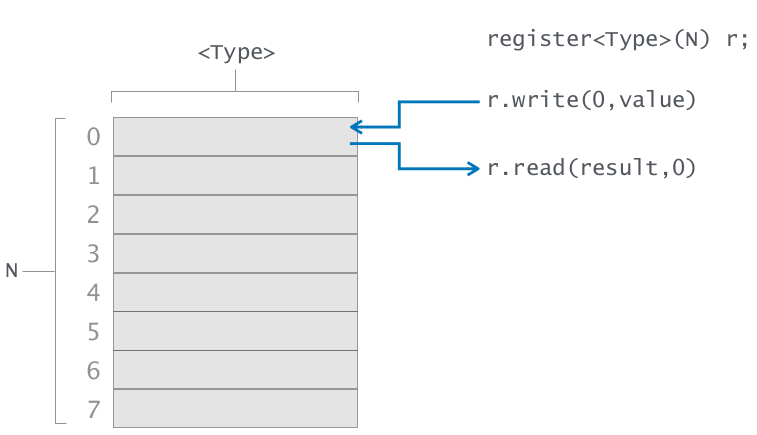
\includegraphics[width=1\textwidth,scale=1]{figures/registers}
		\caption{P4 registers \cite{advnet}}
		\label{fig:registers}
	\end{subfigure}%
	\begin{subfigure}[t]{.33\textwidth}
		\centering
		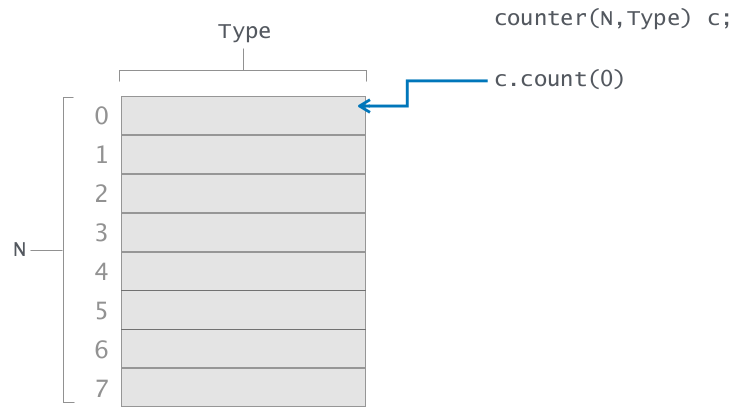
\includegraphics[width=1\textwidth,scale=1]{figures/counters}
		\caption{P4 counters \cite{advnet}}
		\label{fig:counters}
	\end{subfigure}
	\begin{subfigure}[t]{.33\textwidth}
		\centering
		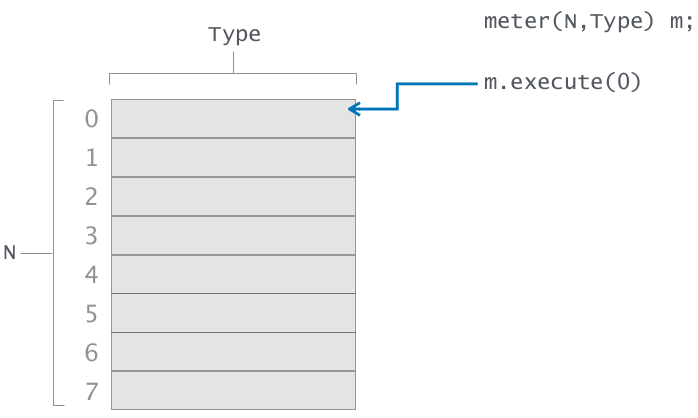
\includegraphics[width=1\textwidth,scale=1]{figures/meters}
		\caption{P4 meters \cite{advnet}}
		\label{fig:meters}
	\end{subfigure}
\end{figure}

\begin{figure}[b!]
	\centering
	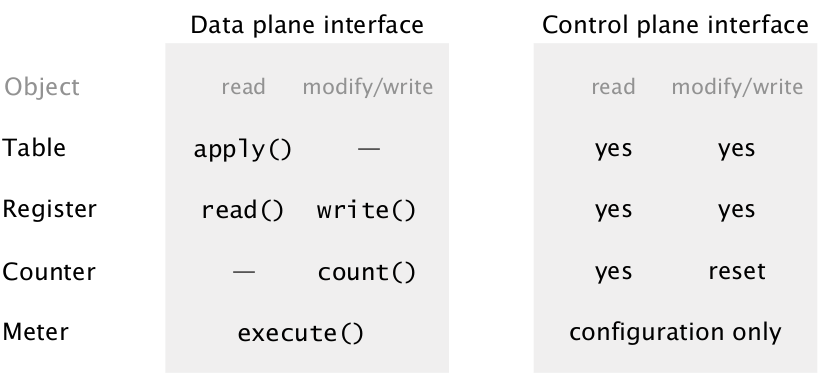
\includegraphics[width=0.6\textwidth,scale=1]{figures/stateful_objects_summary}
	\caption{Stateful objects summary. 	\cite{advnet}}
	\label{fig:stateful_objects_summary}
\end{figure}

\subsection{Hash functions}

P4 \textit{v1model} offers hash functions: \newline
\texttt{enum HashAlgorithm\{crc32,crc32\_custom,crc16,s,random,identity,csum16,xor16\}} \newline
\texttt{extern void hash<O,T,D,M>(out O result, in HashAlgorithm algo, in T base, in D data, in M max);}

\newpage

\section{Probabilistic data structures}

P4 provides us with built-in stateful data structures such as arrays of registers, counters or meters. However, with these we need to deal with severe limitations such as limited number of operations and memory. That's why we consider more advanced stateful data structures.

\subsection{Bloom filter}

We want a data structure for insertion and membership queries. In order to get a deterministic number of required operations, the data structure should be probabilistic. A simple approach would be a basic fixed size table with $M$ 1-bit cells for $N$ elements. If we observe an element, we hash it and set the bit at the corresponding index to 1. Due to hash collision ($N > M$), we get a false positive rate of $FPR = 1 - (1-\frac{1}{M})^N$. The advantage of this approach is that only one operation is required per insertion or query. However, roughly 100x more cells are required than the number of element we want to store for a 1\% false positive rate. \newline

Bloom filters are a more memory-efficient approach for insertions and membership queries. Bloom filters consist of a fixed size table \texttt{bf} with $M$ 1-bit cells and $K$ hash functions and we write a 1 at each position indicate by each hash function.

\begin{figure}[hb]
	\begin{minipage}[t]{.5\textwidth} 
		\vspace{0pt}
		\centering 
		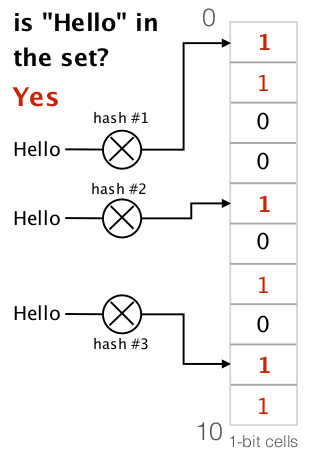
\includegraphics[width=0.45\textwidth]{figures/bloom_filter}
		\caption{Bloom filter. 	\cite{advnet}}
		\label{fig:bloom_filter}
	\end{minipage} 
	\begin{minipage}[t]{.5\textwidth} 
		\vspace{10pt} 
		\begin{itemize}
			\setlength{\itemsep}{0pt}
			\setlength{\parskip}{0pt}
			\item Insert \textit{e} into \texttt{bf}: 
				\begin{enumerate}
					\item $\forall i \in [1,K]$, calculate $h_i(e)$
					\item $\texttt{bf}[h_i(e)] = 1, \forall i \in [1,K]$
				\end{enumerate}
			\item Membership query \textit{e}:
				\begin{enumerate}
					\item if $\texttt{bf}[h_i(e)] == 1, \forall i \in [1,K]$ 
					\newline $\rightarrow$ $e$ is in \texttt{bf}
					\item else 
					\newline $\rightarrow$ $e$ is not in \texttt{bf}
				\end{enumerate}
			\end{itemize}
	\end{minipage} 
\end{figure}

The advantage of bloom filters is that they use about 10x less memory than the simple approach. However, they require slightly more operations.

\subsubsection{Dimension your bloom filter}
\label{bloom_filter_dimension}

$N$ elements, $M$ cells, $K$ hash functions, $FP$ false positive rate.

\vspace{-\topsep}
\begin{itemize}
	\setlength{\itemsep}{0pt}
	\setlength{\parskip}{0pt}
	\item probability that one hash function returns the index of a particular cell: $\frac{1}{M}$
	\item probability that one hash function does not return the index of a particular cell: $1 - \frac{1}{M}$
	\item probability of a cell to be 0: $(1 - \frac{1}{M})^{KN}$
	\item false positive rate P(FP): $(1 - (1 - \frac{1}{M})^{KN})^K$
	\item false negative rate: 0
\end{itemize}
\vspace{-\topsep}

\noindent For an approximation, use: $p := P(FP) = (1 - (1 - \frac{1}{M})^{KN})^K \approxeq (1 - e^{-KN/M})^K$. \newline

\noindent $FN = 0$ since if we have seen an element once, all cells corresponding to its hashes will have been set to 1. Since we never delete elements, $FN = 0$. If we were to delete elements from a bloom filter (i.e. set all cells corresponding to an element to 0), false negatives would be possible.
Because deletions are not possible, the controller may need to regularly reset the bloom filter. Resetting a bloom filter takes some time during which it is not usable. A common trick is to use two bloom filters and use one when the controller resets the other one.

\newpage

\noindent We can't just keep increasing $K$ to lower $FP$ since for too many hash functions, we will have lots of 1s in the table and a lower chance of finding 0s, which increases $FP$. 

\noindent There's a global minimum when $K = \ln(2) * \frac{M}{N}  \approx 0.7*\frac{M}{N}$, found by taking derivative of $P(FP)$. For that choice of $K$, resulting $p := P(FP) = 2^{-K} \approx 0.6185^{M/N}$.\\
Given optimal $K$, choice of optimal $M = -\frac{N \ln p}{(\ln2)^2}$ $\rightarrow O(N)$ space.

\begin{figure}[hb]
	\centering
	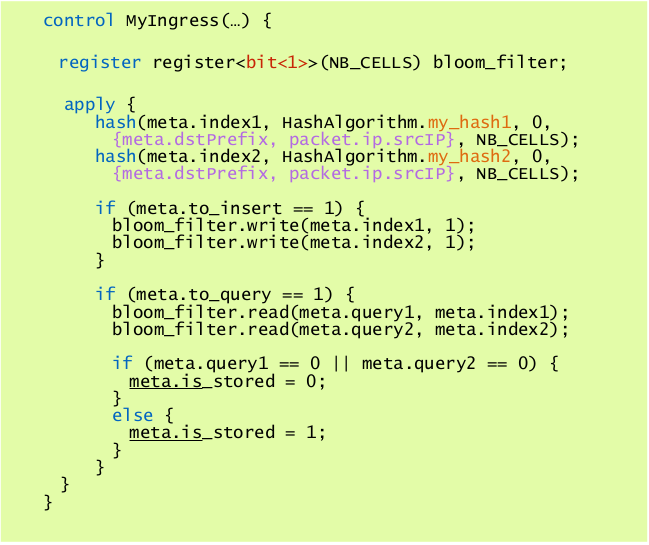
\includegraphics[width=0.55\textwidth,scale=1]{figures/bloom_filter_p4}
	\caption{Bloom filter with $K = 2$ hash functions implemented in $P4_{16}$. \cite{advnet}}
	\label{fig:bloom_filter_p4}
\end{figure}

\subsection{Counting bloom filter}

Since we cannot delete items from a bloom filter, we extend them to handle deletions. For counting bloom filters, to add an element, increment the corresponding counters by 1. The cells are thus no longer 1-bit but larger. To delete an element, decrement the corresponding counters by 1. An element is considered in the table if all counters are larger than 0. All of our prior analysis for standard bloom filters applies to counting bloom filters. We still have $FN = 0$ since a counter of a cell only reaches 0 if all elements mapped to that cell were deleted. Unless we have counter overflow. If a counter gets too large and wraps around to 0, false negatives are possible. Counters must be large enough to avoid overflow. Poisson approximation suggests 4 bits/counter.

Thus, Counting Bloom Filters do handle deletions at the price of using more memory
\vspace{0pt}
\begin{figure}[b!]
	\begin{minipage}[t]{.5\textwidth} 
		\vspace{0pt}
		\centering 
		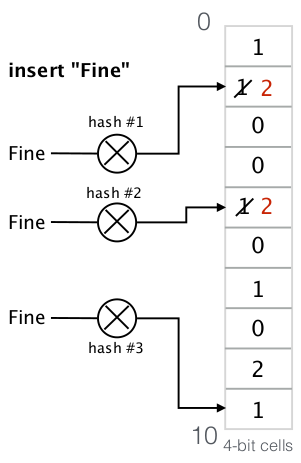
\includegraphics[width=0.45\textwidth]{figures/counting_bloom_filter}
		\caption{Counting bloom filter. \cite{advnet}}
		\label{fig:counting_bloom_filter}
	\end{minipage} 
	\begin{minipage}[t]{.5\textwidth} 
		\vspace{10pt} 
		\begin{itemize}
			\setlength{\itemsep}{0pt}
			\setlength{\parskip}{0pt}
			\item Insert \textit{e} into \texttt{cbf}: 
			\begin{enumerate}
				\item $\forall i \in [1,K]$, calculate $h_i(e)$
				\item $\texttt{cbf}[h_i(e)] \mathrel{+}= 1, \forall i \in [1,K]$
			\end{enumerate}
			\item Membership query \textit{e}:
			\begin{enumerate}
				\item if $\texttt{bf}[h_i(e)] \geq 1, \forall i \in [1,K]$ 
				\newline $\rightarrow$ $e$ is in \texttt{cbf}
				\item else 
				\newline $\rightarrow$ $e$ is not in \texttt{cbf}
			\end{enumerate}
		\end{itemize}
	\end{minipage} 
\end{figure}

\newpage

\subsection{Invertible Bloom Lookup Tables (IBLT)}

Invertible Bloom Lookup Tables (IBLT) stores key-value pairs and allows for lookups and a complete listing. Each cell contains three fields:

\vspace{-\topsep}
\begin{itemize}
	\setlength{\itemsep}{0pt}
	\setlength{\parskip}{0pt}
	\item count: counts the number of entries mapped to this cell
	\item keySum: the sum of all keys mapped to this cell
	\item valueSum: the sum of all the values mapped to this cell
\end{itemize}
\vspace{-\topsep}

\noindent In many settings, we can use XORs in place of sums, for example to avoid overflow issues.

\begin{center}
	\begin{tabular}{ |p{75mm}|p{75mm}| } 
		\hline
		Add a new key-value pair & Delete a key-value pair (assuming it's in set) \\ 
		\hline
		for each hash function & for each hash function\\
		\hspace{3mm} hash the key to find the index & \hspace{3mm} hash the key to find the index \\
		\hspace{3mm} then at this index & \hspace{3mm} then at this index \\
		\hspace{6mm} \textbf{increment} the count by one & \hspace{6mm} \textbf{substract} one from the count \\
		\hspace{6mm} \textbf{add} key to keySum & \hspace{6mm} \textbf{substract} key from keySum \\
		\hspace{6mm} \textbf{add} value to valueSum & \hspace{6mm} \textbf{substract} value from valueSum \\
		\hline
	\end{tabular}
\end{center}

\noindent The value of a key can be found if the key is associated to \textbf{at least} one cell without a hash collision, i.e. a cell with $count = 1$ (see \ref{fig:iblt_lookup}).

\begin{center}
	\begin{tabular}{ |p{100mm}| } 
		\hline
		Listing the IBLT \\
		\hline
		\textbf{While} there is an index for which count = 1 \\
		\hspace{3mm} \textbf{Find} the corresponding key-value pair and return it \\
		\hspace{3mm} \textbf{Delete} the corresponding key-value pair \\
		\hline
	\end{tabular}
\end{center}

\noindent A complete listing is not possible if there is a key that has $count > 1$ at each cell indicated by the hash of the key. Unless the number of iterations is very low, loops can’t be implemented in hardware. The listing is done by the controller.

\begin{figure}[hb]
	\centering
	\begin{subfigure}[t]{.33\textwidth}
		\centering
		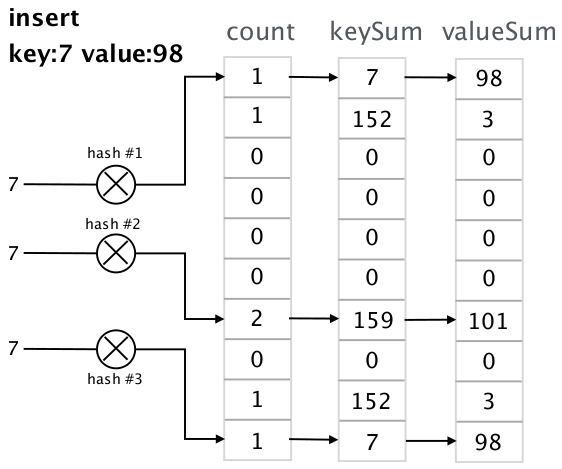
\includegraphics[width=1\textwidth,scale=1]{figures/iblt_1}
		\caption{IBLT insert key:7, value:98}
		\label{fig:iblt_insert}
	\end{subfigure}%
	\begin{subfigure}[t]{.33\textwidth}
		\centering
		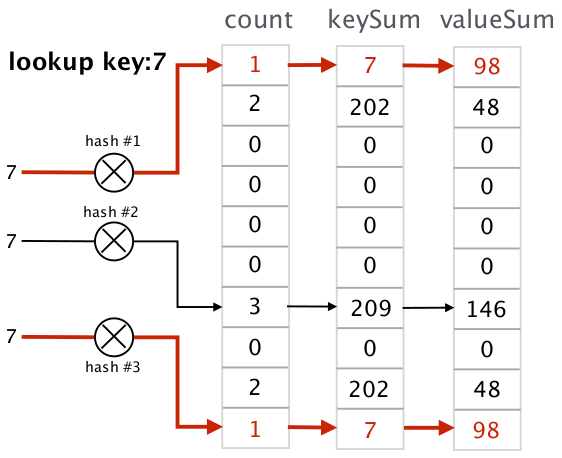
\includegraphics[width=1\textwidth,scale=1]{figures/iblt_2}
		\caption{IBLT lookup key:7}
		\label{fig:iblt_lookup}
	\end{subfigure}
	\begin{subfigure}[t]{.33\textwidth}
		\centering
		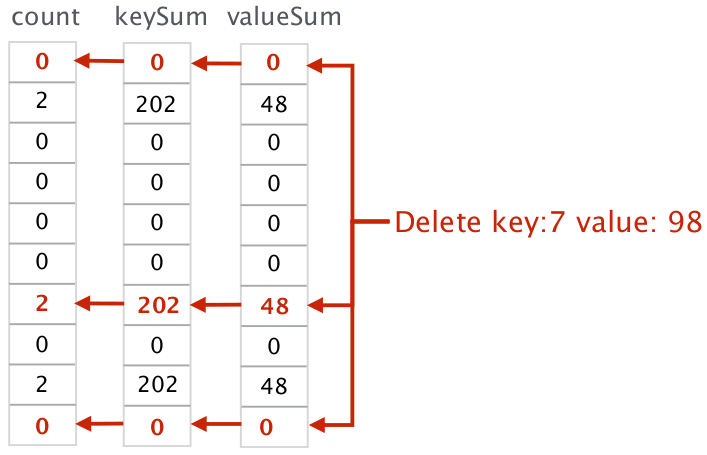
\includegraphics[width=1.25\textwidth,scale=1]{figures/iblt_3}
		\caption{IBLT delete key:7,  value:98}
		\label{fig:iblt_delete}
	\end{subfigure}
	\caption{Invertible Bloom Lookup Tables (IBLT) insertion and lookup \cite{advnet}}
\end{figure}

\newpage

\subsection{Sketches}

Bloom filters allow us to do efficient insertion and membership queries at the cost of false positives. This way we can quickly filter only those elements that might be in the set. However, this is often not enough for monitoring use cases. We also want to approximate frequencies of elements in a data stream. Again, we use probabilistic measures which make this more efficient by allowing miscounting.

\subsubsection{CountMin sketch}

A CountMin sketch uses the same principles as a counting bloom filter, but is designed to have provable L1 error bounds for frequency queries. We use the following notation: a vector of frequencies (counts) of all distinct elements $x_i$: $\vec{x} = [x_1, x_2, ...]^T$.

$$Pr[\hat{x_i} - x_i \geq \epsilon ||\textbf{x}||_1] \leq \delta$$

\noindent with $\hat{x_i}$: estimated frequency, $x_i$: true frequency, $||\textbf{x}||_1$: sum of frequencies.\newline

\noindent A CountMin Sketch uses multiple arrays and hashes. Let $d$ be the number of arrays, with one hash function per array and $w$ indices per array (range of hashes). We thus have $w*d$ counters. CountMin sketches are essentially Bloom filters where we increase the counter at each position indicated by the hashes. Hash collisions can cause over-counting.

\begin{center}
	\begin{tabular}{ |p{75mm}|p{75mm}| } 
		\hline
		Count a new element & Lookup the count of an element \\ 
		\hline
		for each hash function & for each hash function\\
		\hspace{3mm} hash the element to find the index & \hspace{3mm} hash the element to find the index \\
		\hspace{3mm} then at this index & \hspace{3mm} then at this index \\
		\hspace{6mm} \textbf{increment} the count by one & \hspace{6mm} \textbf{lookup} the count \\
		& return the min count \\
		\hline
	\end{tabular}
\end{center}

\begin{figure}[hb]
	\centering
	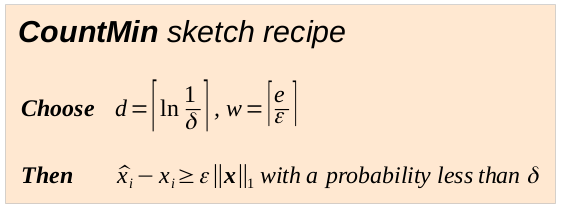
\includegraphics[width=0.5\textwidth,scale=1]{figures/countminsketch_recipe}
	\caption{CountMin sketch recipe, with \textit{e}: Euler's number \cite{advnet}}
	\label{fig:countminsketch_recipe}
\end{figure}

\begin{figure}[b!]
	\centering
	\begin{subfigure}[t]{.5\textwidth}
		\centering
		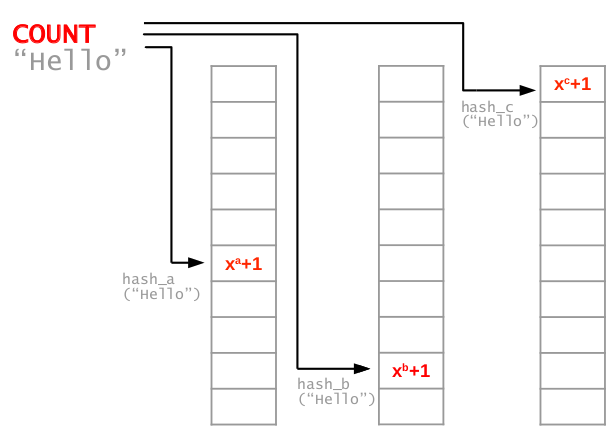
\includegraphics[width=0.7\textwidth,scale=1]{figures/countminsketch_count}
		\label{fig:countminsketch_count}
	\end{subfigure}%
	\begin{subfigure}[t]{.5\textwidth}
		\centering
		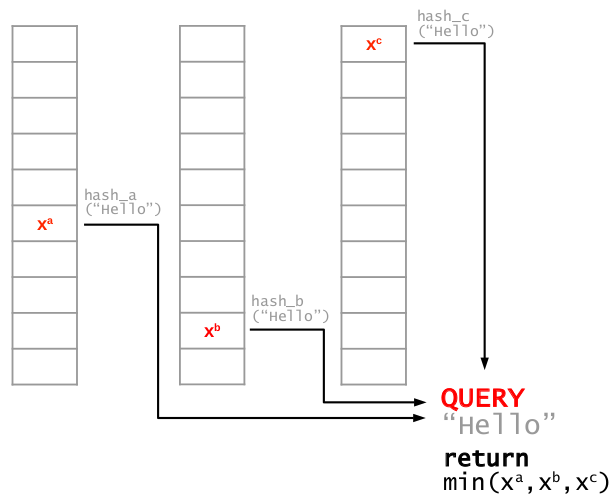
\includegraphics[width=0.7\textwidth,scale=1]{figures/countminsketch_lookup}
		\label{fig:countminsketch_lookup}
	\end{subfigure}
	\caption{CountMin sketches count and lookup \cite{advnet}}
\end{figure}

\newpage

\begin{figure}[t!]
	\centering
	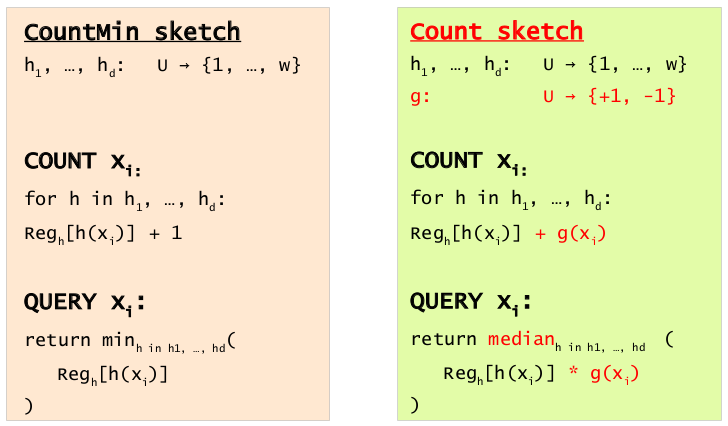
\includegraphics[width=0.7\textwidth,scale=1]{figures/sketches}
	\caption{CountMin sketch and Count sketch \cite{advnet}}
	\label{fig:sketches}
\end{figure}

\subsubsection{Count sketch}

A Count sketch uses the same principles as a counting bloom filter, but is designed to have provable L2 error bounds for frequency queries. The Count sketch uses additional hashing to give L2 error bounds, but requires more resources.

\begin{figure}[hb]
	\centering
	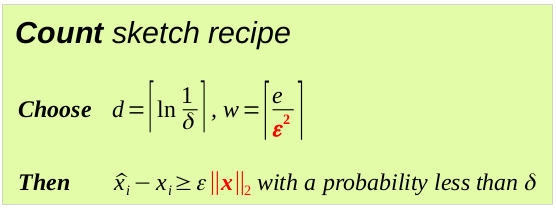
\includegraphics[width=0.5\textwidth,scale=1]{figures/countsketch_recipe}
	\caption{Count sketch recipe \cite{advnet}}
	\label{fig:countsketch_recipe}
\end{figure}

\newpage

\section{P4 hardware targets}

How can we allow network programmability in the field, at reasonable cost, and without sacrificing speed. Let's look at a concrete design: Reconfigurable Match Tables (RMT) \cite{rmt}. This paper argues that flexibility does not come at the price of performance or cost.\\
Let's first look at a fixed-function switch composed of a (de-)parser and a sequence of processing stages. In such a switch, each stage is particularized to its usage. This specificity makes it impossible to trade memory size for another, add a new table, support new headers or new actions.

\begin{figure}[hb]
	\centering
	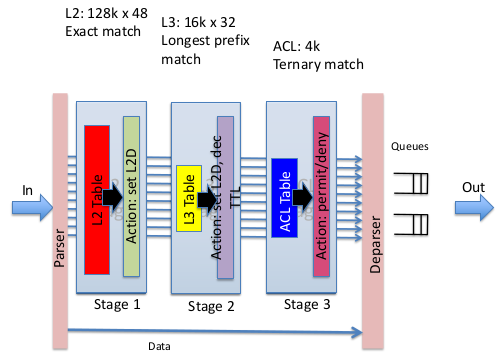
\includegraphics[width=0.5\textwidth,scale=1]{figures/fixed_function_switch}
	\label{fig:fixed_function_switch}
\end{figure}

\noindent SDN wants multiple stages of match-action (flexible allocation), flexible actions and flexible header fields (OpenFlow was designed with these goals in mind). Alternative ways to enable flexibility don't compare in terms of cost-performance ratio: software is 100x too slow and expensive, NPUs are 10x too slow and expensive and FPGAs are 10x to slow and expensive.\\

The solution to all these problems are \textbf{Reconfigurable Match Tables (RMT)}. However, this is challenging to achieve. What kind of switch architecture could support flexibility and yet run at Terabits per second.  At 1Tbps, packet size of 1000bits and 10 operations per packet, we'd need 10 billion operations per second. With a single processor, this would require a 10Ghz processor, which is not feasible. Parallelizing things with a packet-parallel architecture allows to have lower CPU speeds through duplication of the processing units. However, one issue is to scale the memory-to-CPU bandwidth. Replicating memory comes at a huge cost in die area.\\
\noindent The solution is to organize the processing as a pipeline. Pipelined architectures organize processing through a sequence of processing units and local memory. For flexibility, each processing unit/memory can be made generic. Each CPU can process distinct packets, with up to 10 packets going through the pipeline simultaneously.

\begin{figure}[hb]
	\centering
	\begin{subfigure}[t]{.5\textwidth}
		\centering
		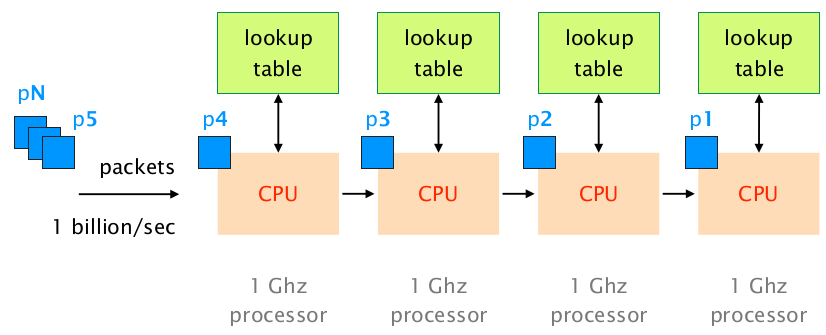
\includegraphics[width=0.9\textwidth,scale=1]{figures/switch_pipeline}
		\caption{Pipeline switch architecture}
		\label{fig:switch_pipeline}
	\end{subfigure}%
	\begin{subfigure}[t]{.5\textwidth}
		\centering
		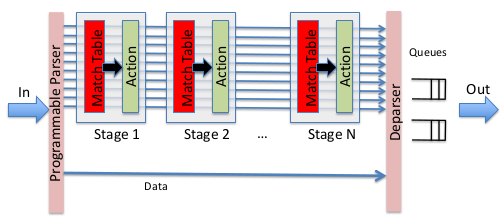
\includegraphics[width=0.9\textwidth,scale=1]{figures/matchaction_forwarding_model}
		\caption{Match/Action Forwarding Model}
		\label{fig:matchaction_forwarding_model}
	\end{subfigure}
\end{figure}

\newpage

\subsection{Parsing}

Parsing is the (complex) process of identifying and extracting the appropriate fields in a packet header. Parsing faces multiple challenges:

\vspace{-\topsep}
\begin{itemize}
	\setlength{\itemsep}{0pt}
	\setlength{\parskip}{0pt}
	\item Throughput: Parser must run at line-rate (parse 1 packet every 70ns on a 10Gbps link)
	\item Dependency: Parsing involves sequential processing as headers typically point to the next
	\item Incompleteness: Some headers do not even identify the subsequent headers
	\item Heterogeneity: Many header formats exist that can appear in various orders/locations
\end{itemize}
\vspace{-\topsep}

\noindent Parse graphs are directed acyclic graphs encoding header types and their sequence. A parser can be divided into two separate blocks: header identification and field extraction. In a programmable parser, the two modules rely on runtime information (stored in memory, e.g. in RAM and/or TCAM) instead of hard-coded logic.

\begin{figure}[hb]
	\centering
	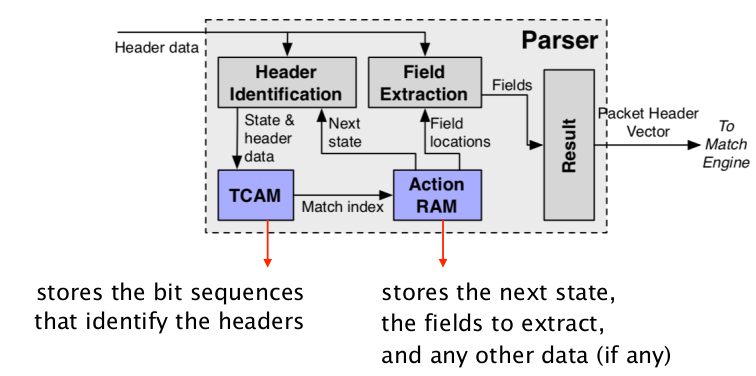
\includegraphics[width=0.7\textwidth,scale=1]{figures/hardware_parser}
	\caption{Programmable hardware parser}
	\label{fig:hardware_parser}
\end{figure}

\subsection{Logical pipeline}

A compiler translates a given RMT logical pipeline (specified in P4) into a physical one. Each physical stage contains dedicated SRAM, for exact matches, and TCAM, for ternary matches. The compiler maps each individual logical stage to one or more physical stage. Small tables can share a stage (up to 16 per stage), while large tables can span multiple ones.\\

\begin{figure}[hb]
	\centering
	\begin{subfigure}[t]{.5\textwidth}
		\centering
		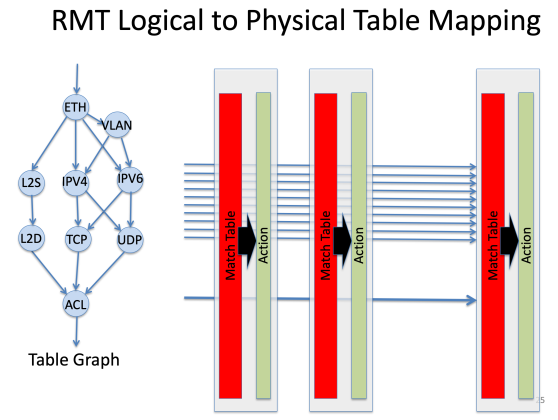
\includegraphics[width=0.9\textwidth,scale=1]{figures/rmt_logical_pipeline}
		\label{fig:rmt_logical_pipeline}
	\end{subfigure}%
	\begin{subfigure}[t]{.5\textwidth}
		\centering
		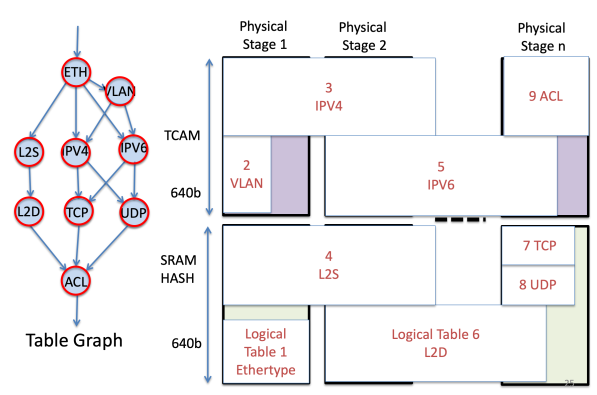
\includegraphics[width=0.9\textwidth,scale=1]{figures/rmt_physical_stages}
		\label{fig:rmt_physical_stages}
	\end{subfigure}
	\caption{Logical pipeline \cite{gibb2013design}}
\end{figure}

\newpage

\noindent The RMT pipeline relies on many Arithmetic Logic Units (ALU) to perform actions on the result of a match. Each ALU modifies only one word of a header (a header is composed of many words). Each stage of the RMT pipeline contains one ALU per word of the header vector (that's a lot of ALUs).

\begin{figure}[hb]
	\centering
	\begin{subfigure}[t]{.5\textwidth}
		\centering
		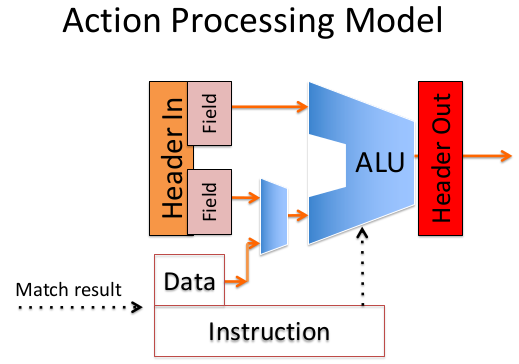
\includegraphics[width=0.7\textwidth,scale=1]{figures/action_processing_model}
		\label{fig:rmt_logical_pipeline}
	\end{subfigure}%
	\begin{subfigure}[t]{.5\textwidth}
		\centering
		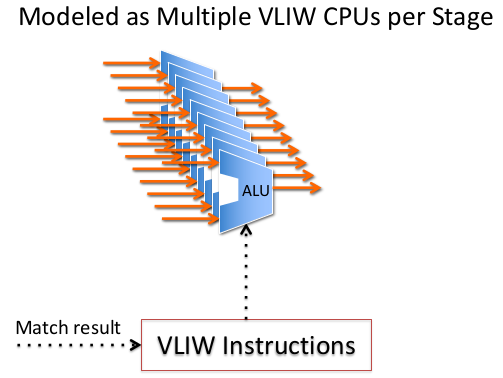
\includegraphics[width=0.7\textwidth,scale=1]{figures/multi_action_processing}
		\label{fig:rmt_physical_stages}
	\end{subfigure}
	\caption{Logical pipeline \cite{gibb2013design}}
\end{figure}

\noindent Building a RMT pipeline is only 15\% more expensive than building a fixed-function switching pipeline. The biggest cost is the memory not the processing logic.\\
In conclusion, we can design a flexible chip using the RMT switch model, bring processing close to the memories (pipeline of many stages) and bring processing to the wires (224 action CPUs per stage). This only causes a 15\% cost increase.

\subsection{Barefoot Tofino}

Barefoot Tofino 6.5 Tbps backplane allows for several billion packets per second at line rate. Tofino relies on Packet Header Vector (PHV) to pass states between stages. Tofino uses four folded match-action pipeline in which the same stages are used for ingress and egress pipeline.

\begin{figure}[hb]
	\centering
	\begin{subfigure}[t]{.5\textwidth}
		\centering
		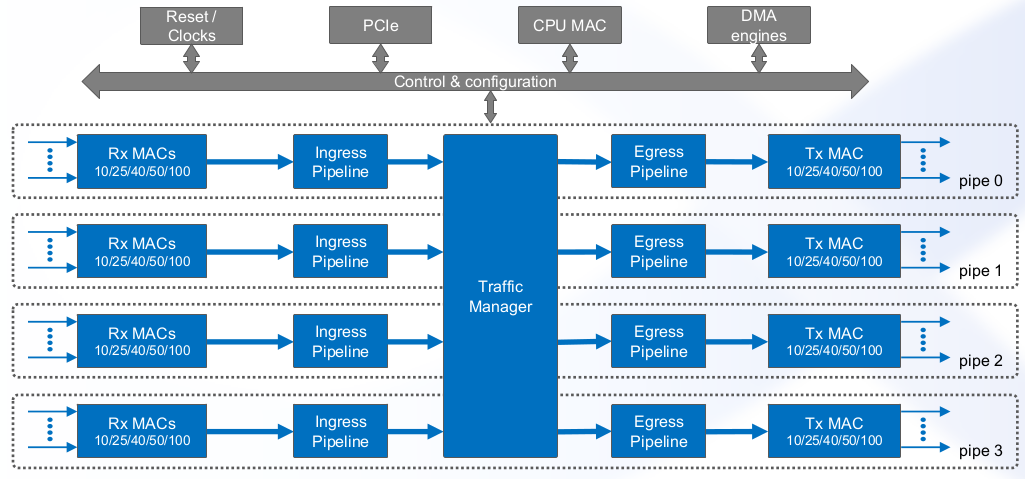
\includegraphics[width=\textwidth,scale=1]{figures/tofino_blockdiagram}
		\label{fig:tofino_blockdiagram}
	\end{subfigure}%
	\begin{subfigure}[t]{.5\textwidth}
		\centering
		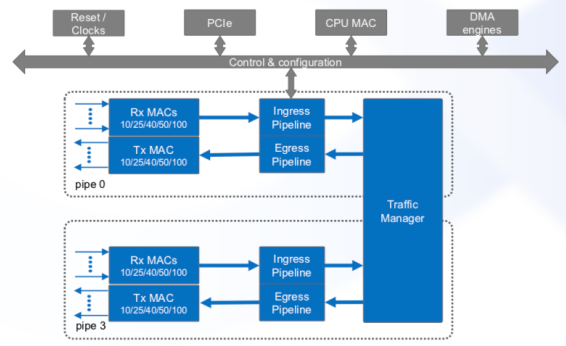
\includegraphics[width=\textwidth,scale=1]{figures/unified_pipeline}
		\label{fig:unified_pipeline}
	\end{subfigure}
	\caption{Barefoot Tofino pipeline \cite{barefoot}}
\end{figure}

\subsubsection{Packet Header Vector (PHV)}

PHVs are a set of uniform containers (8, 16, 32 bit) that carry the headers and metadata along the pipeline. Fields can be packed into any container or their combination. PHV allocation step in the compiler decides the actual packing.

\begin{figure}[hb]
	\centering
	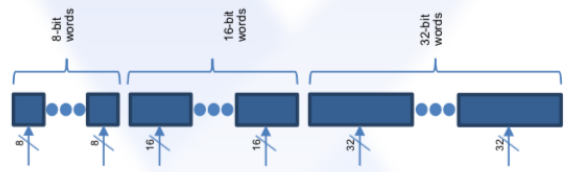
\includegraphics[width=0.3\textwidth,scale=1]{figures/phv}
	\label{fig:phv}
\end{figure}

\subsubsection{Basic structure}

Tofino basically follows the RMT pipeline

\begin{figure}[hb]
	\centering
	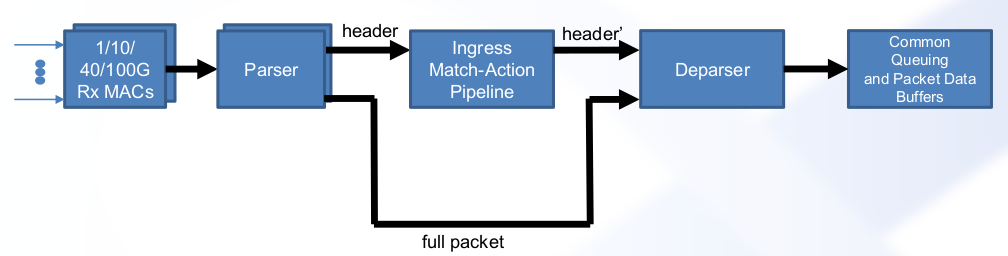
\includegraphics[width=0.6\textwidth,scale=1]{figures/tofino_rmt}
	\caption{Barefoot Networks Tofino basic structure \cite{barefoot}}
	\label{fig:tofino_rmt}
\end{figure}

\begin{figure}[hb]
	\centering
	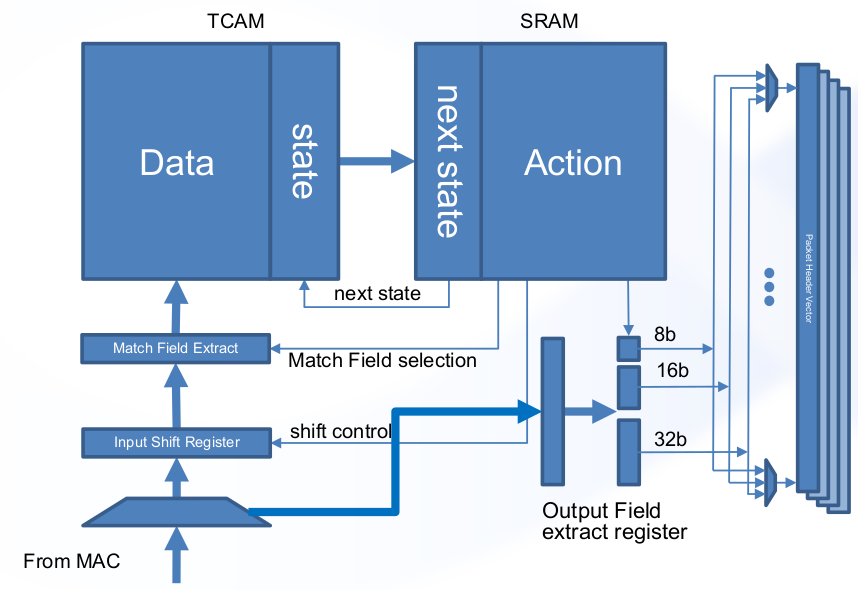
\includegraphics[width=0.7\textwidth,scale=1]{figures/tofino_parser}
	\caption{Barefoot Networks Tofino programmable parser \cite{barefoot}}
	\label{fig:tofino_parser}
\end{figure}

\begin{figure}[b!]
	\centering
	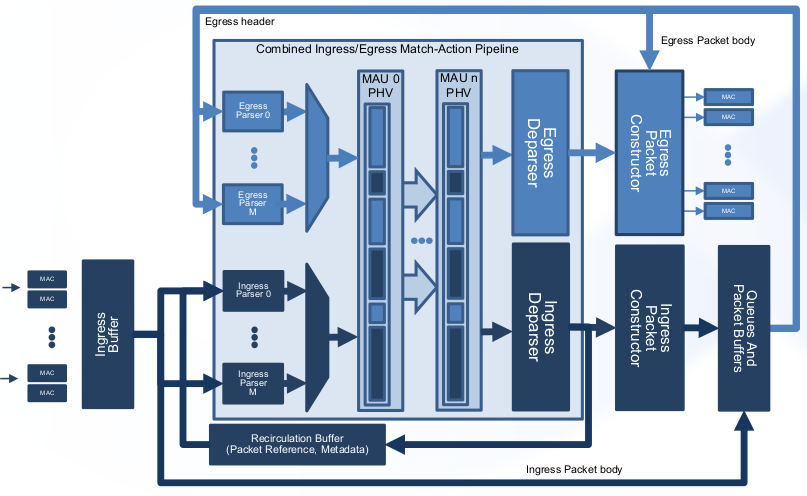
\includegraphics[width=0.8\textwidth,scale=1]{figures/tofino_pipeline}
	\caption{Barefoot Networks Tofino pipeline organization \cite{barefoot}}
	\label{fig:tofino_pipeline}
\end{figure}

\newpage

\noindent Each match action stage is regularly structured around: crossbars, memory units and ALUs.

\begin{figure}[hb]
	\centering
	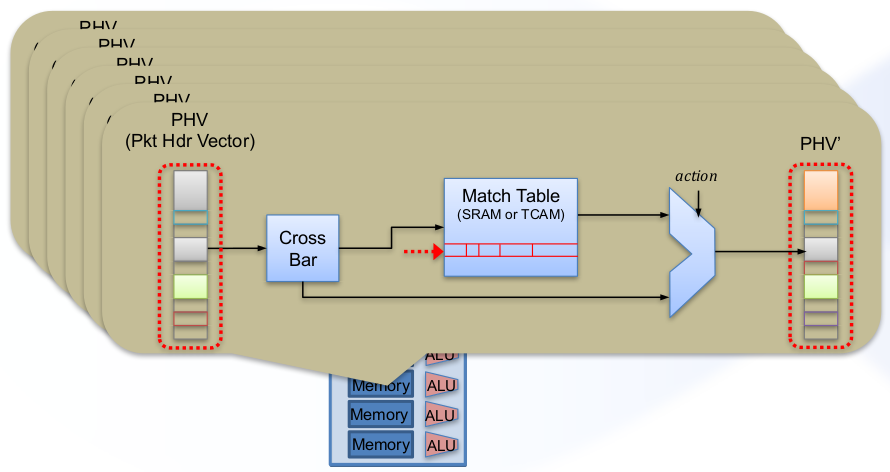
\includegraphics[width=0.7\textwidth,scale=1]{figures/tofino_match_action_stage}
	\label{fig:tofino_match_action_stage}
	\caption{Tofino match action stage \cite{barefoot}}
\end{figure}

\subsubsection{Parallel processing in Tofino}

Most P4 programs have inherent parallelism. In Tofino, multiple tables allow multiple parallel lookups. All actions from all active tables are combined. Each PHV container has its own, independent processor.

\begin{figure}[hb]
	\centering
	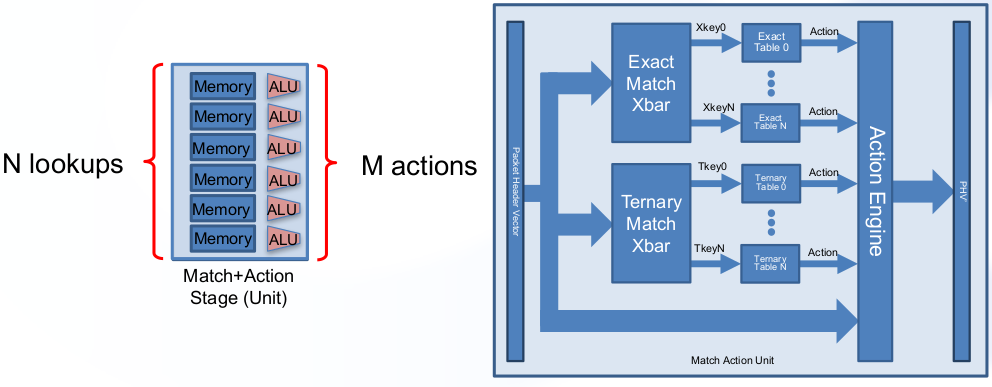
\includegraphics[width=0.7\textwidth,scale=1]{figures/tofino_parallelism}
	\label{fig:tofino_parallelism}
\end{figure}

\begin{figure}[hb]
	\centering
	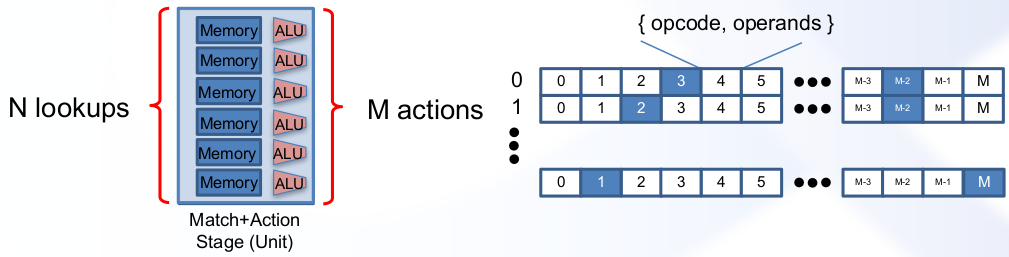
\includegraphics[width=0.7\textwidth,scale=1]{figures/tofino_parallelism_phv}
	\label{fig:tofino_parallelism_phv}
	\caption{How Tofino supports parallelism \cite{barefoot}}
\end{figure}

\newpage

\subsection{P4 switch design}


\begin{itemize}
	\setlength{\itemsep}{0pt}
	\setlength{\parskip}{0pt}
	\item 64 x 10Gb ports (960M packets/second, 1Ghz pipeline)
	\item Programmable parser
	\item 32 match/action stages
	\item Huge TCAM (10x current chips): 64k TCAM words x 640b
	\item SRAM hash tables for exact matches (128k words x 640b)
	\item 224 action processors per stage
\end{itemize}
\vspace{-\topsep}

\section{P4-based applications}

Current research in data plane programmability includes:

\vspace{-\topsep}
\begin{itemize}
	\setlength{\itemsep}{0pt}
	\setlength{\parskip}{0pt}
	\item Data plane programmability for performance, monitoring, applications offloading
	\item Platforms, correctness, management for data plane programmability
\end{itemize}
\vspace{-\topsep}

\noindent A few papers that I found interesting and insightful to read are:

\vspace{-\topsep}
\begin{itemize}
	\setlength{\itemsep}{0pt}
	\setlength{\parskip}{0pt}
	\item Fast network congestion detection and avoidance using P4
	\item Herding the Elephants: Detecting Network-Wide Heavy Hitters with Limited Resources
	\item Network-Wide Heavy Hitter Detection with Commodity Switches
	\item NetPaxos: Consensus at Network Speed
\end{itemize}
\vspace{-\topsep}

\noindent A large set of papers on programmable data planes aim at improving performance, esp. load balancing.

\subsection{CONGA: Distributed Congestion-Aware Load Balancing for Datacenters}

The main thesis of CONGA \cite{conga} is that datacenter load balancing is best done in the network instead of the transport layer, and requires global congestion-awareness to handle asymmetry. Unlike local schemes such as ECMP and Flare, CONGA seamlessly handles asymmetries in the topology or network traffic. CONGA leverages an existing datacenter overlay to implement a leaf-to-leaf feedback loop and can be deployed without any modifications to the TCP stack.\\
CONGA senses the distant drumbeats of remote congestion and orchestrates flowlets to disperse evenly through the fabric. We leave to future work the task of designing more intricate rhythms for more general topologies.

\begin{figure}[hb]
	\centering
	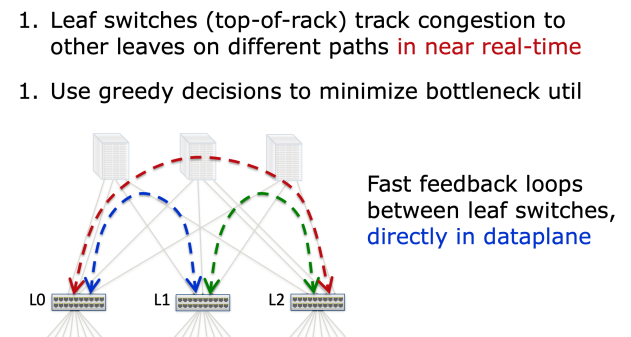
\includegraphics[width=0.5\linewidth]{figures/conga}
	\caption{CONGA: Distributed Congestion-Aware Load Balancing for Datacenters}
	\label{fig:conga}
\end{figure}

\subsection{INT: In-band Network Telemetry}

INT is a mechanism for collecting network state in the dataplane:

\vspace{-\topsep}
\begin{itemize}
	\setlength{\itemsep}{0pt}
	\setlength{\parskip}{0pt}
	\item As close to realtime as possible
	\item At current and future line rates
	\item With a framework that can adapt over time
\end{itemize}
\vspace{-\topsep}

\noindent Examples of network state are: (switch id, ingress port id, egress port id), egress link utilization, hop latency, etc. P4 enables flexible packet parsing and modification for INT. P4 allows INT to adapt to any encapsulation format, any state required to be collected, any feature, protocol (current and future).\\
For example, HULA uses periodic INT probes to disseminate path utilization to switches. Further, flowlet detection and path selection happens at all switches which allows hop-by-hop adaptive routing and load balancing. HULA offers better scalability than CONGA.\\

\noindent In summary, INT provides real-time network state directly in the dataplane while scaling to arbitrarily large networks, scaling to current and future link speeds and being able to adapt to any network, any encap, any application. Knowledge of real-time network state opens up new possibilities such as enhanced monitoring and troubleshooting, network-state aware routing etc.

\subsection{NetCache: Balancing Key-Value Stores with Fast In-Network Caching}

NetCache \cite{netcache} is a rack-scale key-value store that leverages in-network data plane caching to achieve billions QPS troughput with $\approx 10 \mu s$ latency even under dynamic, skewed (i.e. few hot items) workload. It solves the problem of load-balancing in key-values stores observing dynamic, skewed workload. It leverages that a small but very fast cache can provide perfect load-balancing. NetCache relies on the O(billion) throughput of programmable network devices to achieve it in practice. It relies on a tailored UDP-based protocol, an de/encoding scheme for storing variable length values, and sketches. The challenge is to cache the hottest $O(N \log N)$ items with limited insertion rate. The goal is to react quickly and effectively to workload changes with minimal updates.

\subsection{p4v: Practical Verification for Programmable Data Planes}

How do you make sure that a programmable network works as it should? P4 is a low-level language $\rightarrow$ many gotchas. Several problems can arise:

\vspace{-\topsep}
\begin{itemize}
	\setlength{\itemsep}{0pt}
	\setlength{\parskip}{0pt}
	\item header validity: it's hard to always keep validity in your head
	\item unambiguous forwarding: forwarding behavior depends on hardware
\end{itemize}
\vspace{-\topsep}

\noindent Challenges:

\vspace{-\topsep}
\begin{itemize}
	\setlength{\itemsep}{0pt}
	\setlength{\parskip}{0pt}
	\item imprecise semantics: P4 language spec doesn't give precise semantics
	\item modeling the control plane: Table rules are not statically known, populated by the control plane at runtime.
\end{itemize}
\vspace{-\topsep}

\noindent p4v \cite{p4v} is an automated tool for verifying P4 programs. It considers all paths while still being practical for large programs.

\subsection{Others}

\vspace{-\topsep}
\begin{itemize}
	\setlength{\itemsep}{0pt}
	\setlength{\parskip}{0pt}
	\item LossRadar, FlowRadar: Develop techniques and tools to monitor all flows by relying on in-switch data structures (Bloom Filters) and decoding them at the controller-level.
	\item DAPPER, Network-wide HH: Develop P4-based detection mechanisms to diagnose TCP performance issue (e.g. small receiver buffers)	heavy-hitter (e.g. port scanners, superspreader, DDoS).
	\item SketchLearn, ElasticSketch, UnivMon: Introduce techniques to make sketch-based monitoring
	more practical (by making sketches adaptive or "universal")
	\item SwingState: manage programmable network: we need an OS for the data plane! SwingState is a state management framework with 1 primitive: moveStates.
\end{itemize}
\vspace{-\topsep}

\newpage

\section{Exercise design summaries}

\subsection{03-ECMP}
\label{03_ecmp}

Goal: implement ECMP, a very basic (but widely used) technique to load balance traffic across
multiple equal cost paths.

\subsubsection{Data plane}

\vspace{-\topsep}
\begin{itemize}
	\setlength{\itemsep}{0pt}
	\setlength{\parskip}{0pt}
	\item Headers:
	\begin{itemize}
		\setlength{\itemsep}{0pt}
		\setlength{\parskip}{0pt}
		\item Standard ethernet, IP, TCP headers
		\item metadata struct stores ecmp hash and ecmp group id
	\end{itemize}
	\item Parser: Parse ethernet, IPv4, TCP
	\item Ingress:
	\begin{itemize}
		\setlength{\itemsep}{0pt}
		\setlength{\parskip}{0pt}
		\item ipv4\_lpm MAT: matches on the dstIP (lpm). If the dstIP is either directly connected to the switch or there is only one path towards the dstIP, \texttt{set\_nhop()} action is called to just rewrite egress port and MACs. If the dstIP is reachable over \textit{multiple} paths, we call the \texttt{ecmp\_group()} action with the ecmp group id and the number of next hops.
		\item ecmp\_group\_to\_nhop MAT: matches on the ECMP group id and ECMP group hash (exact). Calls \texttt{set\_nhop()}. The rules specify which next hop to choose for which ecmp group id and ecmp hash.
		\item \texttt{set\_nhop()} action: rewrites MACs and egress port, decreases ipv4 TTL
		\item \texttt{ecmp\_group()} action: hashes the flow 5-tuple into meta.ecmp\_hash and stores the ecmp group id in meta.ecmp\_group\_id.
		\item apply: apply forwarding table. In case ecmp\_group was called, apply ecmp\_group\_to\_nhop
	\end{itemize}
	\item Egress: -
	\item Checksum: Since we adapt the packet in set\_nhop (decreasing the ttl), we need to recompute the ipv4 checksum.
	\item Deparser: emit all headers in order
\end{itemize}
\vspace{-\topsep}

\subsection{03-Flowlet-switching}

Goal: ECMP works well for flows with similar size. However, in real traffic flows vary vastly in size. ECMP suffers from performance problems if multiple large flows go through the same path due to hash collisions. We want to fix this by using information from standard\_metadata to fix the collision problem of ECMP by implementing flowlet switching on top of ECMP.

\subsubsection{Data plane}

\vspace{-\topsep}
\begin{itemize}
	\setlength{\itemsep}{0pt}
	\setlength{\parskip}{0pt}
	\item Headers:
	\begin{itemize}
		\setlength{\itemsep}{0pt}
		\setlength{\parskip}{0pt}
		\item Standard ethernet, IP, TCP headers
		\item metadata struct stores ecmp hash and ecmp group id, flowlet last timestamp, flowlet time difference, flowlet register index and flowlet id.
	\end{itemize}
	\item Parser: Parse ethernet, IPv4, TCP
	\item Ingress:
	\begin{itemize}
		\setlength{\itemsep}{0pt}
		\setlength{\parskip}{0pt}
		\item Two registers: \texttt{flowlet\_to\_id} gives the flowlet id for the flowlet register index (hash of the flow 5-tuple). \texttt{flowlet\_time\_stamp} gives the last timestamp for the flowlet register index (hash of the flow 5-tuple).
		\item \texttt{read\_flowlet\_registers} action: hashes the flow 5-tuple, reads the flowlet id and flowlet last timestamp into metadata, updates the timestamp with the current timestamp from standard\_metadata. 
		\item \texttt{update\_flowlet\_id} action: generate a random number and use it as the new flowlet id for the current flowlet (flowlet register index available in metadata)
		\item ipv4\_lpm and ecmp\_group\_to\_nhop MATs as in ECMP
		\item \texttt{set\_nhop()} and \texttt{ecmp\_group()} actions as in ECMP, however the hash in \texttt{ecmp\_group()} now also includes the flowlet id (which periodically changes!)
		\item apply: If IPv4 header is valid, read flowlet registers and update flowlet id incase the flowlet time diff exceeds timeout. Then apply ipv4\_lpm and ecmp.
	\end{itemize}
	\item Egress: -
	\item Checksum: Since we adapt the packet in set\_nhop (decreasing the ttl), we need to recompute the ipv4 checksum.
	\item Deparser: emit all headers in order
\end{itemize}
\vspace{-\topsep}

\subsection{04-CountMin-sketch}

Goal: Implement a CountMin sketch to estimate occurrences of distinct elements.

\subsubsection{Data plane}

\vspace{-\topsep}
\begin{itemize}
	\setlength{\itemsep}{0pt}
	\setlength{\parskip}{0pt}
	\item Headers:
	\begin{itemize}
		\setlength{\itemsep}{0pt}
		\setlength{\parskip}{0pt}
		\item Standard ethernet, IP, TCP headers
		\item metadata struct stores all flow 5-tuple hashes and all counter values read from registers
	\end{itemize}
	\item Parser: Parse ethernet, IPv4, TCP
	\item Ingress:
	\begin{itemize}
		\setlength{\itemsep}{0pt}
		\setlength{\parskip}{0pt}
		\item forwarding MAT: match on ingress port (exact) and rewrite egress port, using \texttt{set\_egress\_port()} action.
		\item Define $N$ registers for CountMin sketch
		\item Define \texttt{sketch\_count()} action that calls a macro for each register. The macro hashes the flow 5-tuple, reads the counter in the registers at the index, increases the counter by 1 and writes back to register.
		\item apply: call \texttt{sketch\_count()} if IPv4 and TCP headers are valid, then apply the forwarding MAT
	\end{itemize}
	\item Egress: -
	\item Checksum: -
	\item Deparser: emit all headers in order
\end{itemize}
\vspace{-\topsep}

\subsubsection{Control plane}

\vspace{-\topsep}
\begin{itemize}
	\setlength{\itemsep}{0pt}
	\setlength{\parskip}{0pt}
	\item Write rules into forwarding MAT
	\item Read registers from control plane (\texttt{self.controller.register\_read()})
	\item Read CountMin sketch by hashing the flow and reading all registers at the specified indices. Return the minimum counter value.
\end{itemize}
\vspace{-\topsep}

\newpage

\subsection{04-Heavy-hitter-detector}

Goal: Use counting bloom filter to estimate heavy hitters.

\subsubsection{Data plane}

\vspace{-\topsep}
\begin{itemize}
	\setlength{\itemsep}{0pt}
	\setlength{\parskip}{0pt}
	\item Headers:
	\begin{itemize}
		\setlength{\itemsep}{0pt}
		\setlength{\parskip}{0pt}
		\item Standard ethernet, IP, TCP headers
		\item metadata struct stores two flow 5-tuple hashes and two counter values read from register
	\end{itemize}
	\item Parser: Parse ethernet, IPv4, TCP
	\item Ingress:
	\begin{itemize}
		\setlength{\itemsep}{0pt}
		\setlength{\parskip}{0pt}
		\item ipv4\_lpm MAT: match on dstIP (lpm) and rewrite MACs and egress port, using \texttt{ipv4\_forward()} action.
		\item \texttt{ipv4\_forward()} action: takes dstMAC and egress port
		\item Define $1$ register for the counting bloom filter
		\item Define \texttt{update\_bloom\_filter()} action that hashes the flow 5-tuple with two different hash functions, writes the hash values in metadata, reads the register at the hash indexes, store theses values in metadata, increase counters and write back to register.
		\item apply: if IPv4 and TCP headers are valid, call \texttt{update\_bloom\_filter()} and drop traffic and return in case both counters exceed a threshold. Apply ipv4\_lpm at the end. 
	\end{itemize}
	\item Egress: -
	\item Checksum: Since we adapt the packet in set\_nhop (decreasing the ttl), we need to recompute the ipv4 checksum.
	\item Deparser: emit all headers in order
\end{itemize}
\vspace{-\topsep}

\subsection{05-Simple-routing}
\label{05-simple-routing}

Goal: implement and provide a control plane to the ECMP routing exercise (see \ref{03_ecmp}). Instead of specifying the entries for the forwarding tables manually, we will now implement a controller that generates and installs forwarding rules automatically, based on the network topology.

\subsubsection{Data plane}

Equivalent to \ref{03_ecmp}.

\subsubsection{Control plane}

\vspace{-\topsep}
\begin{itemize}
	\setlength{\itemsep}{0pt}
	\setlength{\parskip}{0pt}
	\item Iterate over all switches in the topology and connect to them:
	\vspace{-\topsep}
	\begin{lstlisting}
for p4switch in self.topo.get_p4switches():
  thrift_port = self.topo.get_thrift_port(p4switch)
  self.controllers[p4switch] = SimpleSwitchAPI(thrift_port)
	\end{lstlisting}
	\item For each switch (source), iterate over all switch destinations. If the destination is equal to the source, install a ipv4\_lpm table rule for all directly connected hosts. For all other destinations, check the shortest path from source to dst and iterate over all hosts connected to dst. If there is only one single shortest path, install a rule for it in ipv4\_lpm. Otherwise, install a ECMP rule. ECMP groups are defined per switch with the set of next ports. A new ECMP group needs to be created in case the current selection of dst ports does not have an ECMP group yet.
\end{itemize}
\vspace{-\topsep}

\subsection{05-Traceroutable}

Goal: Extend a P4 router with the functionality to respond to traceroute packets, i.e. packets where the IPv4 TTL (time to live) value is equal to 1. If a router receives such a packet, it generates an ICMP Time Exceeded message and sends it back to the original sender of the expired packet.\\
Note: An ICMP header encapsulates the IP and TCP header of the original request.

\subsubsection{Data plane}

\vspace{-\topsep}
\begin{itemize}
	\setlength{\itemsep}{0pt}
	\setlength{\parskip}{0pt}
	\item Headers:
	\begin{itemize}
		\setlength{\itemsep}{0pt}
		\setlength{\parskip}{0pt}
		\item Standard ethernet, IP, TCP headers
		\item new icmp header (8 bytes) with type, code, checksum, unused
		\item headers struct contains icmp and two ipv4 headers (the original one and the one added by ICMP, ipv4\_icmp). The ipv4\_icmp header is going to be the ipv4 header of the ICMP packet with the actual src and dst. The original ipv4 header (ipv4 header of the packet that triggered the ICMP response) is going to be encapsulated in the ICMP header (unchanged). 
		\item metadata struct stores ecmp hash and ecmp group id
	\end{itemize}
	\item Parser: Parse ethernet, IPv4, TCP
	\item Ingress:
	\begin{itemize}
		\setlength{\itemsep}{0pt}
		\setlength{\parskip}{0pt}
		\item ipv4\_lpm, ecmp\_group\_to\_nhop MATs as in ECMP
		\item set\_nhop, ecmp\_group actions as in ECMP
		\item icmp\_ingress\_port MAT: matches on the ingress port and calls action set\_src\_icmp\_ip. The reason for this table is when sending back an ICMP reply, we need to set the srcIP of the ICMP packet. We set it to the IP of the interface on which we send out the packet. This table will be populated by the controller.
		\item set\_src\_icmp\_ip: takes an IP address as parameter and sets the hdr.ipv4\_icmp.srcAddr to it.
		\item apply: If the ipv4 header is valid and $ttl > 1$, we simply apply the ipv4\_lpm table and do ECMP if the ecmp\_group action was run (see \ref{03_ecmp}). If ipv4 and tcp headers are valid \textit{and} ttl == 1, we need to respond with an ICMP packet. We thus set the icmp and ipv4\_icmp headers to valid, and prepare the packet to be sent back as ICMP packet: set egress port to ingress port, swap MACs, copy the original ipv4 header into the ipv4\_icmp header, set its dstAddr to the srcAddr and apply the icmp\_ingress\_port MAT (i.e. setting the srcIP to the interface IP). Finally, set the protocol field of ipv4\_icmp to ICMP, adapt the ttl and adapt the totalLen. Set the ICMP type and code and truncate the packet.
	\end{itemize}
	\item Egress: -
	\item Checksum: since we have three different headers (ipv4\_icmp, icmp, ipv4) that all include checksums and all headers can be changed, we have to recalculate the checksum for each header.
	\item Deparser: emit ethernet, ipv4\_icmp, icmp, ipv4, tcp
\end{itemize}
\vspace{-\topsep}

\newpage

\subsubsection{Control plane}

\vspace{-\topsep}
\begin{itemize}
	\setlength{\itemsep}{0pt}
	\setlength{\parskip}{0pt}
	\item Write rules into ipv4\_lpm MAT
	\item Write ECMP rules as explained in section \ref{05-simple-routing}
	\item For each switch, for each interface on it, write an entry into icmp\_ingress\_port MAT.
	\vspace{-\topsep}
	\begin{lstlisting}
for sw_name, controller in self.controllers.items():
  for intf, node in self.topo.get_interfaces_to_node(sw_name).items():
    ip = self.topo.node_to_node_interface_ip(sw_name, node).split("/")[0]
    port_number = self.topo.interface_to_port(sw_name, intf)

    self.controllers[sw_name].table_add("icmp_ingress_port", 
    "set_src_icmp_ip", [str(port_number)], [str(ip)])
	\end{lstlisting}
\end{itemize}
\vspace{-\topsep}

\subsection{06-Packet-Loss-Detection}

Goal: Implement LossRadar. Packet losses are very common in nowadays networks. Those losses can be caused by many reasons: congestion, blackholes, faulty links or corrupted forwarding tables. LossRadar uses two IBLTs for each unidirectional link: one upstream meter for the sending switch, one downstream meter for the receiving switch. To make sure that the meters that are exchanged where exposed to the exact same set of packets batches are used. Lost packets can be detected by taking the difference between the UM and the DM, i.e. substract the counts and xor the values. This will be done by the controller. The controller will be informed by a copy-to-cpu packet which includes a loss header with the last batch id.

\subsubsection{Data plane}

\vspace{-\topsep}
\begin{itemize}
	\setlength{\itemsep}{0pt}
	\setlength{\parskip}{0pt}
	\item Headers:
	\begin{itemize}
		\setlength{\itemsep}{0pt}
		\setlength{\parskip}{0pt}
		\item Standard ethernet, IP, TCP, UDP headers
		\item loss header (batch\_id, padding, nextProtocol), will be between IP and TCP/UDP header, thus we need a nextProtocol field
		\item headers struct contains ethernet, ipv4, loss, tcp, udp
		\item metadata struct stores tmp\_src\_port, tmp\_dst\_port (since we have TCP and UDP, we need uniform reference to the port), 3 hash value fields for the UM, 3 hash value fields for the DM, temp srcIP, dstIP, ports\_proto\_id, counter for updating the IBLT, fields with last local, previous and current batch id and an indicator whether to exectute DM, UM.
	\end{itemize}
	\item Parser: Parse ethernet, IPv4, loss, TCP/UDP
	\item Ingress:
	\begin{itemize}
		\setlength{\itemsep}{0pt}
		\setlength{\parskip}{0pt}
		\item forwarding MAT that calls set\_egress\_port action (set correct egress port)
		\item remove\_loss\_header MAT that calls remove\_header action (if the link goes toward a host we need to remove the loss header)
		\item 8 registers: one each srcIP, dstIP, (ports, proto, id), counter; for both UM and DM
		\item compute\_hash\_indexes() action: calculates hash indexes for all three hash functions on flow 5-tuple into metadata with correct bounds for both UM and DM.
		\item \texttt{apply\_um\_meter()} action: increases counter and xors value in UM registers at all indexes indicated by hashes
		\item \texttt{apply\_dm\_meter()} action: increases counter and xors value in DM registers at all indexes indicated by hashes
		\newpage
		\item apply: get L4 ports in metadata, add loss header if not present (assumes that we have no host-switch-host connections) - else store batch id as previous batch id, read last local batch id and update batch id. If new batch id is different from last local batch id, inform controller. Update batch id in loss header. Compute hashes and remove loss header if necessary. Apply UM (if flag to not execute is not set), apply DM (if flag to not execute is not set). Finally, drop packet if ttl=1, otherwise decrease ttl by 1.
	\end{itemize}
	\item Egress: if the packet is a clone packet, set loss header valid, ipv4 invalid, set batch id as last local batch id and set etherType.
	\item Checksum: Update checksum of ipv4
	\item Deparser: emit ethernet, ipv4, loss, tcp, udp
\end{itemize}
\vspace{-\topsep}

\subsubsection{Control plane}

\vspace{-\topsep}
\begin{itemize}
	\setlength{\itemsep}{0pt}
	\setlength{\parskip}{0pt}
	\item Write rules into forwarding MAT
	\item set crc custom hashes
	\item Upon receiving a clone packet:
	\begin{itemize}
		\item Get the loss header fields (batch id) and the switch name (src)
		\item Iterate over all neighboring switches (dst) of the switch (src)
		\item For each neighboring switch, check the link to it: get the ports of the link at each respective switch, the extract the registers for both switches (UM for src, DM for dst).
		\item Decode the two IBLTs: first, take the difference between UM and DM (UM-DM) (subtract counters and xor values) and store in diff array. Then, while there is a counter==1 in the counter diff array, get the array index associated with that counter and read out srcIP, dstIP, (ports, proto, id) in the respective diff arrays. From this, you get the flow 5-tuple. This allows you to calculate all 3 hashes for the flow. Then, at the 3 positions in the diff arrays indicated by the hashes, decrease the counter by 1 and xor the values with the values of the found flow 5-tuple. The found flow is a dropped packet.
	\end{itemize}
\end{itemize}
\vspace{-\topsep}

\begin{figure}
	\centering
	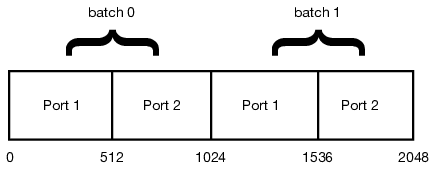
\includegraphics[width=0.7\linewidth]{figures/ex06-register-structure}
	\caption{Register port and batch structure}
	\label{fig:ex06-register-structure}
\end{figure}


\newpage

\section{Oral exam questions}

\noindent \textbf{What is P4? What does it enable?}

P4 is a programming language that allows us to program reprogrammable switches. It tries to achieve reconfigurability, protocol independence and target independence. Rather than have the switch tell us the limited set of things it can do, P4 gives us a way to tell the switch what it should do, and how it should process packets.
P4 enables us to define custom protocols by defining parsers and let's us control switches "top-down" by first specifying their forwarding behavior, then populating the tables we've defined. Instead of the switch chip vendor defining our API for us, and locking us into using their next chip as well, P4 let's us define the API we need to populate the switch. We say that P4 is "top-down" because it puts the network architect, programmer, and developer in charge, rather than the chip vendor.
As such, we can define our own protocols and don't have to rely on hardware vendors to include protocols, as it was the case with OpenFlow. In OpenFlow, each supported protocol needs to be specified since OpenFlow assumes fixed-function switch chips.\\

\noindent \textbf{What are the main differences between OpenFlow and P4?}

\textit{OpenFlow is an API to the data plane, P4 allows to program the data plane.}

\noindent  P4 is \textit{not} a replacement for OpenFlow - they try to achieve different things. Both are focused on opening up the forwarding plane. OpenFlow tries to centrally and remotely control lots of different switches, essentially providing an API to directly access the data plane. P4 on the other hand addresses a different need in the network, the need to \textit{program} the data plane.\\
OpenFlow assumes the switch to have a fixed, well-known behavior, typically described in the datasheet of the switch ASIC. These switches supported a fixed set of protocols and you couldn't change their behavior or add new protocols. As interest in OpenFlow grew, more and more header-types were added. However, adding your own protocol is essentially only possible if you are a company with big influence and smaller companies are bound to use existing protocols. Adding more and more protcols led to OpenFlow becoming an "overblown beast". This strange behavior is all caused by the fact that switches were not programmable.\\
That's where P4 comes in. With programmable switches, we can simply tell the switch how to process packets and what tables to keep. Programmers could define whatever API made sense to populate the tables they created in the switches. And that exactly is what P4 does. P4 is a common language to specify how a switch should process packets. P4 lets us define what headers a switch will recognize (or "parse"), how to match on each header, and what actions we would like the switch to perform on each header.\\

\newpage

\noindent \textbf{What roles do tables, actions and control flow play in P4?}

Tables, actions and control flow are all components of P4 that play together for packet processing. P4 is based on the reconfigurable match tables (RMT) model. Once a packet has been parsed, it is matched against a set of tables. 

\vspace{-\topsep}
\begin{itemize}
	\setlength{\itemsep}{0pt}
	\setlength{\parskip}{0pt}
	\item Tables: A table matches on a set of header fields and applies an action with specified parameters. A match-action table entry thus consists of a set of header fields to match and a set of action parameters. Matching can be done in different ways (exact, lpm, ternary, range).
	\item Action: An action is essentially a \textit{function} as known from classical programming languages. Actions can modify the packets and can be either invoked from within the control block or as a result of a match in a match-action table.
	\item Control flow: Control flow allows us to specify how a packet is processed, specifying in what order tables and actions are applied. We can run actions, apply a table, check if a table has matched, which action was run, etc.
\end{itemize}
\vspace{-\topsep}

\noindent \textbf{What different memory structures exist in P4 switches? How do they differ?}

We know that P4 switches make packet processing more efficient by making use of pipelined architectures that organize processing through a sequence of processing units and local memory. Match-action tables and parsers both need efficient memory lookups for matching. However, different matching types require different kinds of memory. As such, P4 switches have two different types of memory: TCAM and SRAM.

\vspace{-\topsep}
\begin{itemize}
	\setlength{\itemsep}{0pt}
	\setlength{\parskip}{0pt}
	\item \textbf{SRAM(input: address, output: data)}: SRAM allows for fast random access, however it is expensive. As such, SRAM is used for exact matching in match action tables and to store the next state, fields to extract and other data (if any) for parsing.
	
	\begin{itemize}
		\item Exact match MAT: In an exact match, we want to lookup the action for exact match-key data. We can use Cuckoo hashing to get $O(1)$ worst-case lookup, deletion and average-case insertion. For exact matching we hash the match-key and then do an SRAM lookup.
		\item Parsing: The SRAM stores next state information, fields to extract, and any other data needed during parsing.
	\end{itemize}	
	
	\item \textbf{TCAM(input: match field value, output: address of action)}: TCAM (ternary content-addressable memory) is a specialized type of high-speed memory that searches its entire contents in a single clock cycle. Generally speaking, CAM is often described as the opposite of random access memory (RAM). To retrieve data on RAM, the operating system (OS) must provide the memory address where the data is stored. Data stored on CAM can be accessed by performing a query for the content itself, and the memory retrieves the addresses where that data can be found. Due to its parallel nature, CAM (and by extension TCAM) is much faster than RAM. CAM is essentially a massively parallel lookup engine that searches all entries in parallel and selects the best match in constant time. The term “ternary” refers to the memory's ability to store and query data using three different inputs: 0, 1 and X. The “X” input, which is often referred to as a “don’t care” or “wildcard” state, enables TCAM to perform broader searches based on pattern matching (a binary CAM matches	every bit precisely).
	
	\begin{itemize}
	\item LPM/ternary match MAT: In an LPM match, we want to lookup the action with the most specific match for a match-key. As such, SRAM is not ideal since we have multiple possible memory locations (a key can match several patterns). This is where TCAM comes into play: TCAM matches the key against all entries and returns the action address of the best match.
	\item Parsing: The TCAM stores bit sequences that identify headers. The current state and a subset of bytes from the buffer are sent to the TCAM, which returns the first matching entry. The output of the TCAM points to an SRAM entry which specifies
	the next state for the header identification module and the headers that were matched. The RAM entry may also specify data such as the number of bytes to advance and the subset of bytes to extract next (see figure \ref{fig:hardware_parser}).
	\end{itemize}	
\end{itemize}
\vspace{-\topsep}

\noindent \textbf{What types of constructs do we need to maintain state across packets?}

In P4, variables have local scope and their value is not maintained across subsequent invocations for different packets. However, there is a need for stateful programming (e.g. think of a stateful firewall).\\
P4 offers 4 different types of stateful objects: registers, counters and meters.

\vspace{-\topsep}
\begin{itemize}
	\setlength{\itemsep}{0pt}
	\setlength{\parskip}{0pt}
	\item Registers: Registers are arrays of bit vectors. Both the width of the bit vector and the length of the array can be specified. Registers are stateful - they maintain their value across packets. We can read from and write to a specified register index. Registers can also be read from the control plane.
	
	\item Counters: Counters are used for counting. Counters are assigned in arrays and an index needs to be specified when executing a \texttt{count()} operation. Counters can be increased from the data plane but can only be read from the control plane. Counters can be one of three different types: packets, bytes, packet\_and\_bytes. There also exist direct counters which can be directly attached to a MAT.
	
	\item Meters: Meters are used for rate-limiting. Meters are also assigned in arrays. Like counters, we also have direct meters that can be attached to MATs.
	\item MATs: Match-action tables can also be used to maintain state.\\
\end{itemize}
\vspace{-\topsep}

\noindent \textbf{What is a bloom filter? How do you dimension one?}

A bloom filter is a probabilistic data structure that is used for membership queries. A Bloom filter enables a deterministic number of required operations at the cost of false positives. A Bloom filter consists of a fixed-size array (size M) of 1-bit cells and $K$ hash functions for insertion of $N$ elements. Inserting an element consists of hashing the element with all hash functions and setting the 1-bit cell to 1 at each position indicated by the $K$ hash functions. To check if an element is in the Bloom filter, we hash the element with each Hash function and check the 1-bit cells indexed by the hashes. If all cells are 1, we declare the element to be in the filter, else it's not in the filter. Due to hash collisions, we can get false positives, i.e. in the case where element $e_1$ has a hash collision with element $e_2$ on all $K$ hash functions: 

$$h_i(e_1) = h_i(e_2) \qquad \forall i \in [1,K]$$

\noindent Given $N, M$, we can design a Bloom Filter with minimal false positive rate by choosing 

$$K = ln(2) * \frac{M}{N}$$

\noindent (see section \ref{bloom_filter_dimension})\\

\noindent \textbf{Explain what is a counter and the different ways it can be used.}

Counters are one out of three stateful objects in P4. Counters are used for counting (obviously) and are always assigned in arrays. Counters can be one of three different counting types: packets, bytes, packets\_and\_bytes. Further, there are two different counter types: indirect and direct counters. We can call \texttt{count()} from the data plane but counters can only be read from the control plane.
\vspace{-\topsep}
\begin{itemize}
	\setlength{\itemsep}{0pt}
	\setlength{\parskip}{0pt}
	\item Indirect counter: Indirect counters are arrays of n\_counters independent counter values. Calling \texttt{count(in S index)} will increase the counter at the specified index.
	\item Direct counter: Direct counters are counters that are directly attached to tables.\\
\end{itemize}
\vspace{-\topsep}

\newpage

\noindent \textbf{Describe the role of the 'register' extern in the v1model and how it can be used (at a high level).}

Registers are one out of three stateful objects in P4. Registers are useful for storing (small amounts of) arbitrary data. Registers are assigned in arrays for which we can specify the length and width. We can read and write from/to registers from the data plane as well as from the control plane. This sets them apart from counters which can only be read from the control plane. As such, registers are widely used to store data that must be available over subsequent packets.\\
Further, registers play an important role when creating more complex data structures such as Bloom filters or CountMin sketches.\\


\noindent \textbf{In the exercise we made a 'traceroutable' P4 network. To do that we needed to generate ICMP packets when the TTL expired. Explain which additions were needed? (header definitions, how did the main headers struct look like, parser, main ingress/ egress logic, checksum updates, etc).}

ICMP packets consist of an ethernet header, IP header and ICMP header. Inside the ICMP header, we have the original IP and TCP headers of the packet that created the ICMP message.

\vspace{-\topsep}
\begin{itemize}
	\setlength{\itemsep}{0pt}
	\setlength{\parskip}{0pt}
	\item Headers: ICMP header (8 bytes total: type, code, checksum, unused), ipv4\_icmp headers which is a normal ipv4 header.
	\item Main headers struct: the main headers struct thus included the following structs: ethernet (ethernet header), ipv4\_icmp (ipv4 header), icmp (icmp header), ipv4 (ipv4 header), tcp (tcp header)
\end{itemize}
\vspace{-\topsep}

\noindent The parser remained unchanged since we only sent out ICMP packets. In the Deparser, we had to add two additional emits, essentially emitting all headers in the right order: ethernet, ipv4\_icmp, icmp, ipv4, tcp.\\
For the ingress, we needed one additional table which matches on the ingress port and then sets the srcIP of the ipv4\_icmp to the IP of the interface. In the ingress logic, we have to differentiate between $ttl > 1$, in which case we apply normal forwarding/ECMP, and $ttl == 1$. For the later, we first set the ipv4\_icmp and icmp headers to valid. We then adapt the packet headers such that the packet can be sent back out on the port it came in (i.e. switch MACs, set egress port to ingress port, set dstIP to srcIP). We then apply the aforementioned table to set the srcIP of the ipv4\_icmp header to the IP of the interface.

\newpage

\noindent \textbf{Desing question}

\begin{figure}[hb]
	\centering
	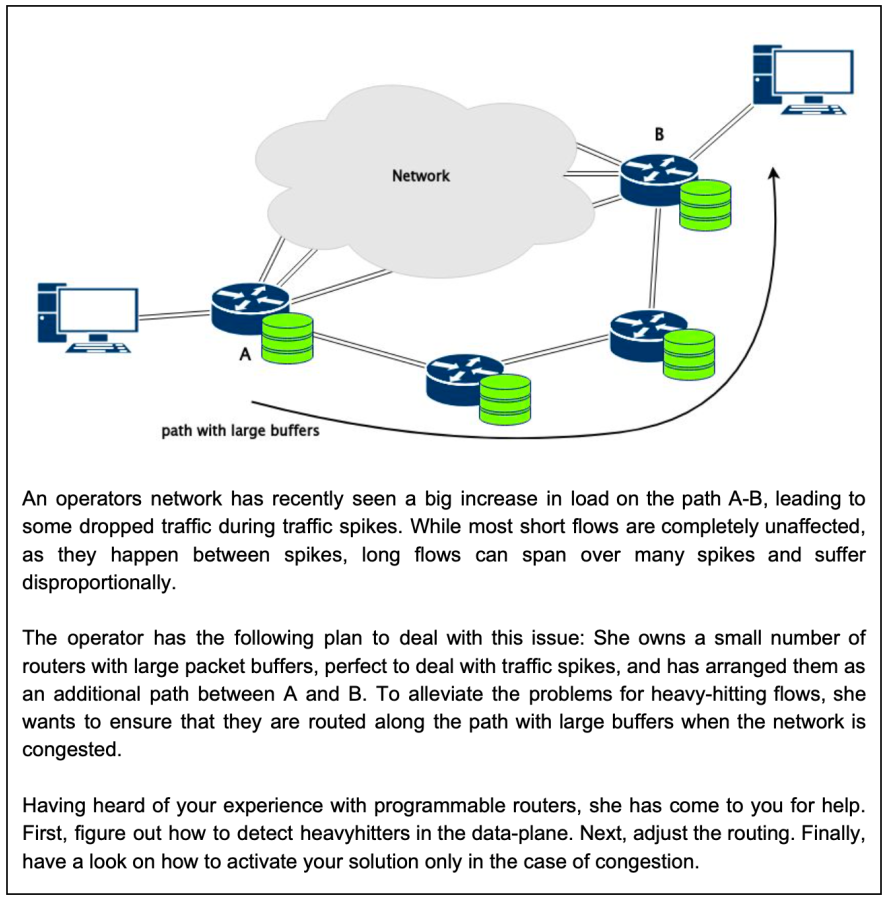
\includegraphics[width=0.8\linewidth]{figures/design_question}
	\label{fig:designquestion}
\end{figure}

There are three parts to this system design that need to be specified: the heavy hitter detection, the routing change and how to only activate the solution in case of congestion.

\vspace{-\topsep}
\begin{itemize}
	\setlength{\itemsep}{0pt}
	\setlength{\parskip}{0pt}
	\item Heavy hitter detection: all flows enter the network through a single switch $A$. Thus no distributed detection technique is necessary. We can thus use a CountMin sketch to estimate the number of packets in a flow. The \texttt{count()} action is called for every valid packet in the ingress.
	\item Routing change: We can use two different ipv4\_lpm MATs: a 'normal' MAT ipv4\_lpm that routes traffic through the standard network and a buffer MAT ipv4\_lpm\_buffer that send incoming traffic at $A$ over the large buffer path. Both MATs match on the dstIP (lpm) and the action sets the next hop by rewriting the egress port and the dstMAC. The next hops of the ipv4\_lpm MAT are inside the network whereas the next hop of the ipv4\_lpm\_buffer MAT is the next large buffer switch after A. In the apply section of the ingress, we first increase the CountMin sketch and then compare the counts (stored in a metadata field) against a pre-specified threshold. If all counts exceed the threshold, we have a heavy hitter and apply the ipv4\_lpm\_buffer MAT which will set the next hop to a large bufffer router. Else we apply the ipv4\_lpm MAT. This approach does the routing change fully in the data plane, thus there is no induced latency by control plane communication. However, we do need to maintain two MATs which wastes memory.
	\item Activation: In order to only activate the solution in case of congestion, we need to observe some congestion signals to actually detect congestion. 
\end{itemize}
\vspace{-\topsep}

\label{lastpage} % this must stay here
\clearpage
\addcontentsline{toc}{section}{References}
\bibliographystyle{acm}
\bibliography{refs}

\clearpage
\appendix
\pagenumbering{Roman}

\end{document}
